% This template originates from the Cambridge University thesis 
% which is created by Prof Harish Bhanderi.  
% This is template follows the GNU license for Education and training
% purposes. (http://www-h.eng.cam.ac.uk/help/tpl/textprocessing/ThesisStyle/) 
% 
%
% I modified for uses in University of Information Technology 
% Vietnam National University. 

\documentclass[oneside,12pt]{Classes/uitBA}
 \ifpdf
     \pdfinfo { /Title  (Nghien cuu ky thuat va xay dung ung dung tim kiem doi tuong tren anh)
                /Creator (TeX)
                /Producer (pdfTeX)
                /Author (Nguyen Van Bien, Pham Duy)
                /CreationDate (D:20140601000000)  %format D:YYYYMMDDhhmmss
                /ModDate (D:20030815213532)
                /Subject (Thesis title)
                /Keywords (PhD, Thesis)}
     \pdfcatalog { /PageMode (/UseOutlines)
                   /OpenAction (fitbh)  }
 \fi
     
  \university{{ĐẠI HỌC QUỐC GIA THÀNH PHỐ HỒ CHÍ MINH}}
  \collegeordept{{ĐẠI HỌC CÔNG NGHỆ THÔNG TIN\\
  					KHOA KHOA HỌC MÁY TÍNH}}  
  
  \author{{NGUYỄN VĂN BIÊN - 10520245 
           \\PHẠM DUY - 10520074}}    
  
  \title{NGHIÊN CỨU KỸ THUẬT
  	\\VÀ XÂY DỰNG ỨNG DỤNG
  	\\TÌM KIẾM ĐỐI TƯỢNG TRÊN ẢNH} 
  	
  %\crest{
\includegraphics[scale=.30]{UITLogo}} 
           
  \degree{CỬ NHÂN NGÀNH KHOA HỌC MÁY TÍNH\\}  
  
  \supervisor{{TS. NGÔ ĐỨC THÀNH 
  			 \\PGS. TS. LÊ ĐÌNH DUY}}
  \degreedate{TP. HỒ CHÍ MINH, 2014} 
\hbadness=10000
\hfuzz=50pt
\usepackage{StyleFiles/watermark}
\onehalfspacing

 
%% Load the package with the acronym option
\usepackage{hyperref}
\usepackage{acronym}

%subscript
\usepackage{fixltx2e}

\begin{document}
\maketitle
\setcounter{secnumdepth}{3}
\setcounter{tocdepth}{3}

\frontmatter % book mode only
\pagenumbering{roman}
% 
\begin{dedication}  

Xin dành tặng quyển luận văn này cho ... 

\end{dedication}

 
 
 
\begin{acknowledgements}      

Tôi xin chân thành cám ơn ... 

\end{acknowledgements}
  
 
\begin{abstracts}         




\end{abstracts}
 

\tableofcontents
\listoffigures
\listoftables

% Add acronyms
%\newpage
%\documentclass[a4paper,12pt]{article}
%\usepackage{hyperref}
%\usepackage{acronym}

\chapter*{Danh mục từ viết tắt}

\printnomenclature  
\addcontentsline{toc}{chapter}{Danh sách từ viết tắt}

\begin{acronym}
\acro{BoW}{Bag-of-Words} 
\acro{SPM}{Spatial Pyramid Matching } 

\end{acronym}

%\printnomenclature  
%\addcontentsline{toc}{chapter}{THUAT NGU}




\mainmatter  
% \pagebreak[4]
% \hspace*{1cm}
% \pagebreak[4]
% \hspace*{1cm}
% \pagebreak[4]

\chapter{Giới thiệu tổng quan}
\ifpdf
    \graphicspath{{Chapter1/Chapter1Figs/PNG/}{Chapter1/Chapter1Figs/PDF/}{Chapter1/Chapter1Figs/}}
\else
    \graphicspath{{Chapter1/Chapter1Figs/EPS/}{Chapter1/Chapter1Figs/}}
\fi
\markboth{\MakeUppercase{\thechapter. Giới thiệu tổng quan}}{Chương \thechapter. Giới thiệu tổng quan}
\section{Mục tiêu và động lực chọn đề tài}
Trong những năm gần đây, cùng với sự phát triển của công nghệ thông tin, các lĩnh vực liên quan đến kỹ thuật số cũng đang có tốc độ phát triển chóng mặt. Các thiết bị kỹ thuật số như máy ảnh, máy quay phim kỹ thuật số, camera số, điện thoại di động có chức năng chụp hình, ... đang ngày càng phổ biến và không ngừng gia tăng về số lượng. Chính điều này đã làm sản sinh ra một lượng thông tin số khổng lồ bao gồm hình ảnh, video, v.v... Do đó, nhu cầu truy vấn thông tin từ kho dữ liệu hình ảnh, video ngày càng bức thiết hơn bao giờ hết.\\
Mục tiêu của luận văn này nhằm xây dựng một hệ thống truy vấn ảnh trên tập dữ liệu lớn, trong đó quá trình truy vấn hoàn toàn dựa trên nội dung của ảnh và kết quả phải được trả về gần như ngay lập tức với cơ sở dữ liệu gồm hàng triệu hình ảnh chưa được gán nhãn. Hệ thống này tập trung vào giải quyết vấn đề về tìm kiếm một đối tượng cụ thể như một địa điểm, một bức tranh, một bìa sách, v.v... Những đối tượng này có thể được chụp trong các điều kiện khác nhau như góc chụp, ánh sáng, kích thước hay bị che khuất. Do đó mục đích của hệ thống không phải là trả về những hình ảnh chụp gần giống nhau như chụp trong cùng một khung cảnh mà là trả về những hình ảnh có chứa đối tượng cần tìm. Ví dụ như khi đưa vào một bức hình có chứa Nhà thờ Đức Bà, kết quả trả về sẽ những bức hình có chứa nhà thờ Đức Bà chứ không phải trả về những nhà thờ có kiến trúc gần giống với Nhà thờ Đức Bà.\\
Những hệ thống truy vấn ảnh trên tập dữ liệu lớn có rất nhiều ứng dụng trong thực tế. Chúng tôi sẽ liệt kê sơ lược một vài ứng dụng trong phần tiếp theo.\\

\section{Một vài hướng ứng dụng thực tế của hệ thống}

Trong cuộc sống, ta có thể dễ dàng bắt gặp những ứng dụng vô cùng hữu ích của các hệ thống truy vấn đối tượng trên ảnh. Dưới đây là một vài hướng ứng dụng cụ thể:\\
\textbf{Nhận dạng đối tượng, sản phẩm.} Với sự phổ biến của điện thoại thông minh và internet, một người có thể dễ dàng dùng điện thoại chụp một tấm hình và hỏi hệ thống về thông tin của đối tượng trong tấm hình đó. Ví dụ, tại một cửa hàng, một người mua hàng có thể tham khảo giá của một sản phẩm tại các cửa hàng khác; trong thư viện, một độc giả có thể tìm được những cuốn sách nào chứa hình ảnh mình quan tâm; khi đi thăm bảo tàng, du khách có thể tìm kiếm thêm thông tin về một hiện vật trong đó, v.v...\\
\textbf{Nhận dạng địa điểm.} Vị trí địa lý của nơi chụp tấm hình cũng có thể được xác định bằng việc truy vấn thông tin của đối tượng trong hình từ những cơ sở dữ liệu lớn chứa hình ảnh và thông tin vị trí như Google Street View hay kho hình ảnh có lưu kèm thông tin GPS. Hệ thống này có thể là một giải pháp thay thế rẻ tiền cho các thiết bị có GPS. Chẳng hạn, khi một du khách đến một nơi mà anh ta chưa bao giờ đặt chân tới nhưng lại không GPS hay bản đồ, anh ta có thể chụp một tấm hình của một tòa nhà hay những cảnh tại nơi đó để xác định được vị trí chính xác của mình.\\
\textbf{Tìm kiếm và quản lý kho dữ liệu video.} Hàng ngày, một lượng lớn dữ liệu video được sinh ra và ta không thể nào quản lý hết được nội dung của chúng. Ví dụ, một đài truyền hình muốn tìm kiếm tất cả các đoạn quảng cáo có liên quan đến một nhãn hiệu sản phẩm mà họ đã từng phát trong vài năm gần đây, một hệ thống truy vấn ảnh sẽ dễ dàng thực hiện điều này chỉ với một hình ảnh của sản phẩm.\\
\textbf{Gán nhãn ảnh tự động.} Những tấm ảnh có thể được gán nhãn một cách tự động về địa điểm hay đối tượng trong hình để dễ dàng cho việc tìm kiếm và quản lý sau này. Ví dụ, người dùng có thể dễ dàng tìm kiếm được những bức hình chụp tại một địa điểm nào đó mà không cần biết nó nằm trong album nào hay được chụp ngày nào. Những hệ thống lớn lưu trữ ảnh lớn như của Facebook có thể dễ dàng phát hiện và gán nhãn khuôn mặt người nhưng vẫn chưa thể nhận dạng được địa điểm mà tấm hình được chụp từ nội dung chứa trong hình.\\
\textbf{Sử dụng trong quảng cáo theo ngữ cảnh.} Rất nhiều công ty quảng cáo đặt màn hình tại nơi công cộng để quảng cáo cho các sản phẩm của mình nhưng các quảng cáo này chưa thực sự hướng người dùng và kém hiệu quả. Việc sử dụng một hệ thống có thể quảng cáo theo ngữ cảnh và hướng đúng đối tượng người dùng sẽ giúp việc quảng cáo hiệu quả hơn. Ví dụ, một camera trong thang máy có thể tự động phát hiện được những sản phẩm người đi thang máy đang dùng như nhãn hiệu chai nước họ đang uống, nhãn hiệu quần áo họ đang mặc,... để lựa chọn được những quảng cáo phù hợp với đối tượng người dùng và phát trên màn hình.\\
\textbf{Tăng tính tương tác thực tế.} Với sự ra đời của các sản phẩm công nghệ gần gũi với cuộc sống như Google Glass, việc nhận dạng đối tượng trong thời gian thực sẽ mang đến nhiều thông tin hữu ích cho người dùng.\\
\textbf{Hỗ trợ cho các hệ thống thị giác máy tính khác.} Hệ thống truy vấn đối tượng có thể được dùng để hỗ trợ cho các hệ thống thị giác máy tính khác. Một ví dụ điển hình là hệ thống tự động tái tạo hình ảnh ba chiều sẽ cần gom cụm các hình ảnh của cùng một đối tượng từ một tập dữ liệu lớn.\\

\section{Những thách thức đặt ra}
 Để giải quyết bài toán truy vấn đối tượng trên tập dữ liệu ảnh lớn, có rất nhiều thách thức được đặt ra. Dưới đây chúng tôi sẽ trình bày một vài thách thức trong bài toán này:\\
 \begin{figure}[!htbp]
  \begin{center}
    \leavevmode
    \ifpdf
      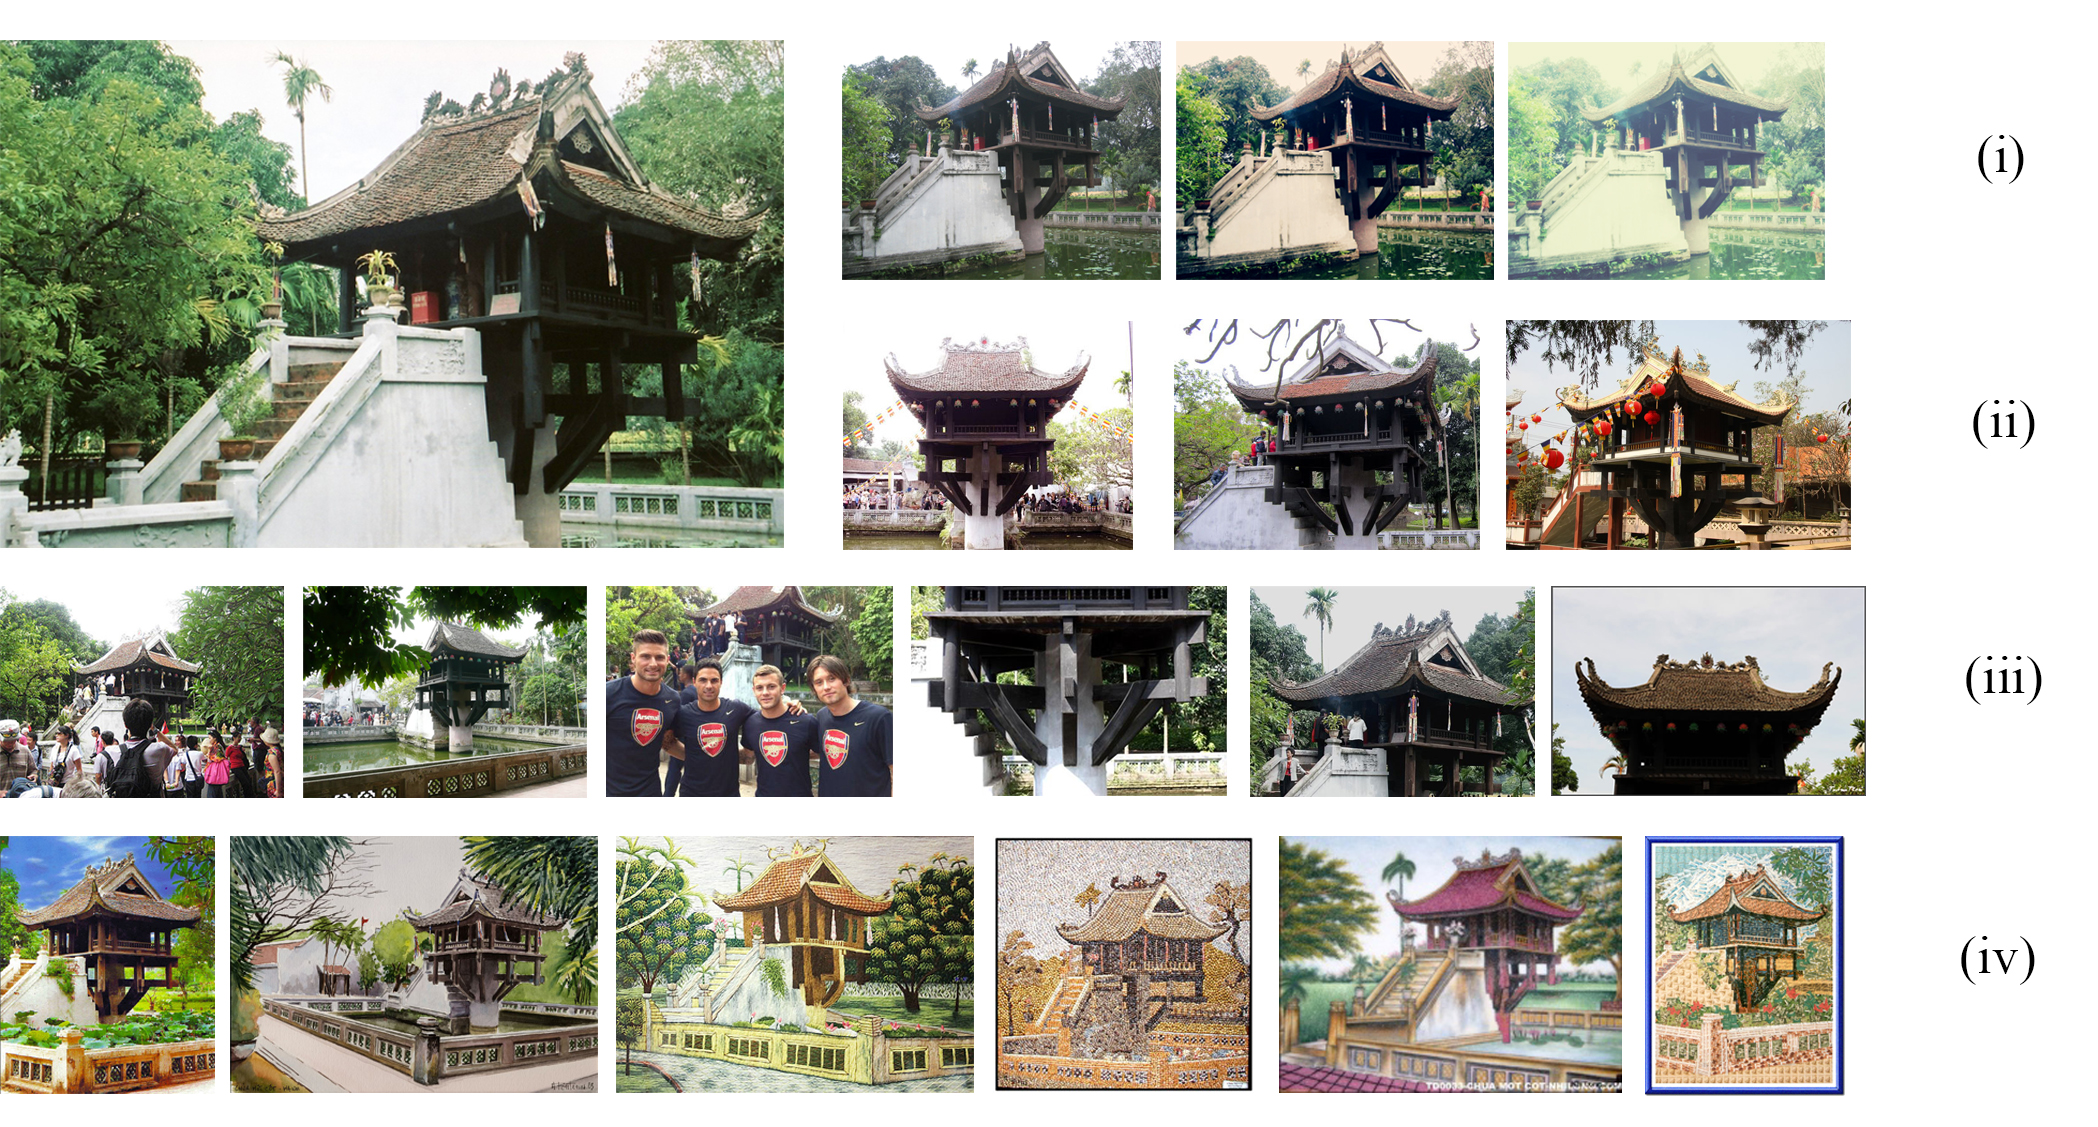
\includegraphics[scale=0.20]{chuaMotCot}
    \else
      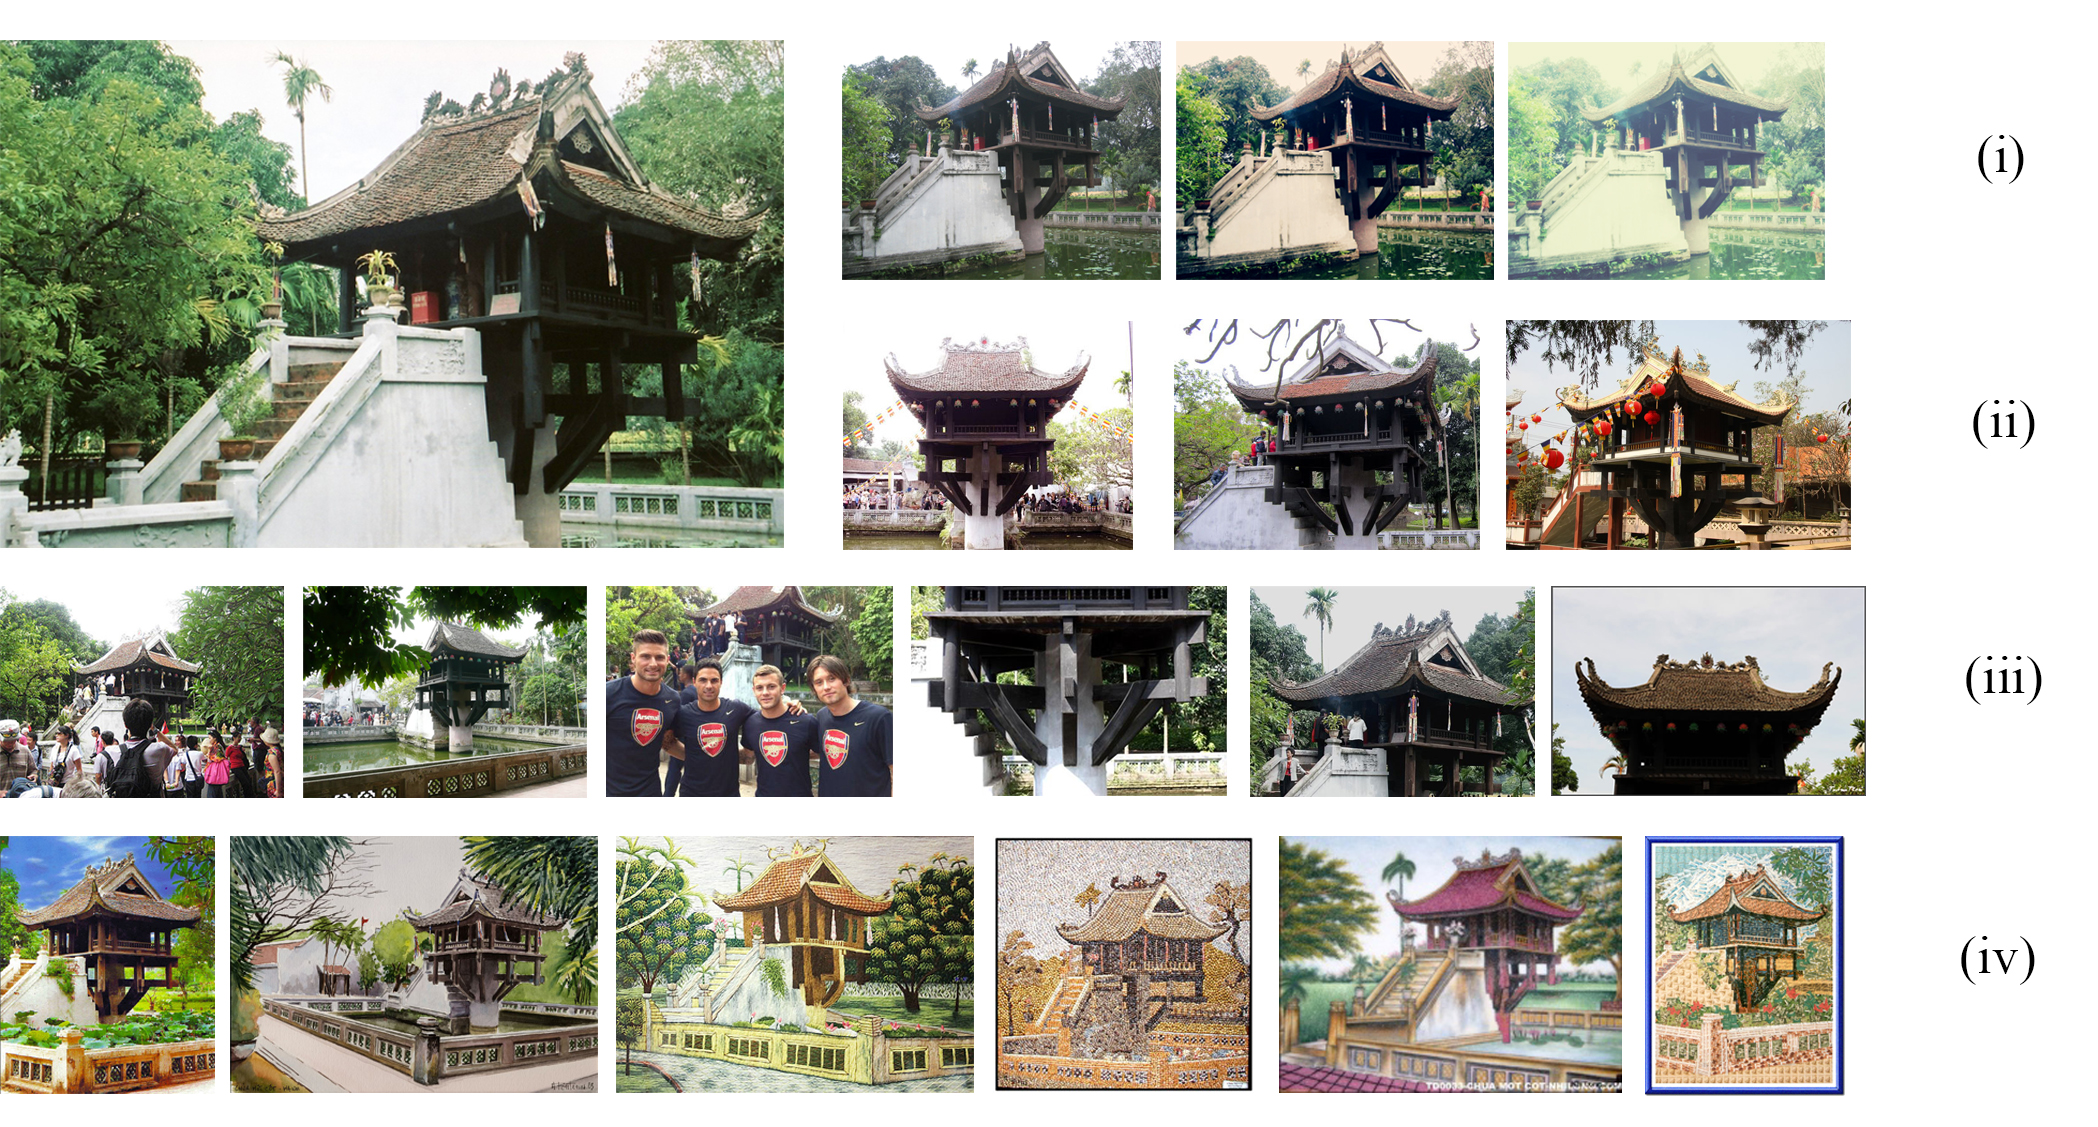
\includegraphics[scale=0.20]{chuaMotCot}
    \fi
    \caption[Những thay đổi bề ngoài của đối tượng trên ảnh]{\textbf{Những thay đổi bề ngoài của đối tượng trên ảnh.} \textit{(i) Hình ảnh đối tượng trong các điều kiện chiếu sáng khác nhau. (ii) Hình ảnh đối tượng dưới các góc chụp khác nhau. (iii) Đối tượng bị che khuất hay hình ảnh đối tượng bị cắt ghép. (iv) Hình ảnh đối tượng trong các ấn phẩm, bản in, bản vẽ.}}
    \label{FigTemple}
  \end{center}
\end{figure} 
 \textbf{Sự biến đổi bề ngoài của đối tượng trong hình ảnh.} Một hệ thống truy vấn đối tượng trên hình ảnh cần phải trả về được các hình ảnh có chứa đối tượng quan tâm bất chấp mọi thay đổi trên bên ngoài của đối tượng. Những thay đổi đó có thể đến từ rất nhiều nguyên nhân khác nhau. Đó có thể do tác động từ các yếu tố bên ngoài khi chụp hình như điều kiện chiếu sáng, góc chụp của camera hay những tùy chỉnh khác nhau của các camera về độ tương phản, độ phân giải, màu sắc,... Cùng với đó là những hình ảnh của đối tượng được chụp với góc xoay, kích thước hình hay tỉ lệ khác nhau. Hoặc có những trường hợp đối tượng bị che khuất, cắt ghép, v.v... hoặc đối tượng được thể hiện trên các ấn phẩm, bản in, bản vẽ nên bị thay đổi về màu sắc và chi tiết. Một vài dạng thay đổi kể trên được thể hiện qua Hình \ref{FigTemple}. Còn một trường hợp nữa là do những thay đổi từ chính bản thân đối tượng do các điều kiện bên ngoài ví dụ như đối tượng bị cũ đi hay bị xuống cấp theo thời gian.\\ 
 \textbf{Các loại đặc tính vật lý khác nhau trên mỗi đối tượng.} Dựa trên các đặc tính vật lý người ta chia đối tượng thành các loại khác nhau. Có những đối tượng mà đặc tính thể hiện rõ nét nhất qua cấu trúc bề mặt, nhưng có cái lại qua màu sắc hay hình dạng, v.v... Ví dụ như với những con bướm, đặc trưng cho chúng không phải là hình dạng, kích cỡ vì đa phần các loài bướm đều có hình dạng, kích cỡ gần giống nhau mà ở đây là các họa tiết, màu sắc trên cánh bướm; Hay với những loại lá cây thì đặc trưng về màu sắc, họa tiết lại không cung cấp nhiều thông tin bằng hình dạng của lá.\\
 \textbf{Kích cỡ của tập dữ liệu lớn.} Tập dữ liệu hình ảnh lớn thường bao gồm hàng triệu bức ảnh, vậy nên để người dùng có thể tương tác trực tiếp với hệ thống thông qua một thiết bị phía client như điện thoại di động thì đòi hỏi truy vấn phải được trả về trong thời gian ngắn chấp nhận được. Do đó cần phải có một thuật toán nhận dạng hiệu quả, chi phí thấp. Đồng thời những hình ảnh cũng phải được xử lý để lưu trữ sao cho tiết kiệm nhất để phù hợp với kích cỡ của RAM vì nếu lưu trữ trên ổ cứng sẽ mất rất nhiều thời gian để truy xuất và không thể đạt được yêu cầu về thời gian.\\

\section{Cấu trúc luận văn}
Trong phần này, chúng tôi sẽ trình bày cấu trúc phần còn lại của luận văn và những vấn đề được thảo luận ở phần kế tiếp. Các nội dung sẽ được trình bày ở phần kế tiếp bao gồm:\\
 \textbf{Các công trình liên quan.} Chúng tôi sẽ giới thiệu tổng quát về các công trình nghiên cứu liên quan tới truy vấn ảnh và bàn luận chi tiết về từng công trình trong Chương 2.\\
 \textbf{Các tập dữ liệu và phương pháp đánh giá.} Để thử nghiệm kết quả của phương pháp đề xuất và so sánh hiệu suất của chúng với những phương pháp khác, chúng tôi thử nghiệm trên 3 bộ dữ liệu chuẩn là Oxford 5k, Paris 6k và Holiday. Kết quả sẽ được đánh giá bằng phương pháp mean Average Precision (mAP). Chi tiết của mỗi bộ dữ liệu cùng phương pháp đánh giá sẽ được trình bày chi tiết ở Chương 3.\\
 \textbf{Tích hợp thông tin không gian ảnh vào phương pháp đánh chỉ mục ngược.} Chúng tôi đề xuất một phương pháp nhằm nâng cao hiệu suất của các hệ thống truy vấn đối tượng bằng cách tích hợp thông tin không gian ảnh vào phương pháp đánh chỉ mục ngược (inverted index). Trong Chương 4, chúng tôi sẽ trình bày chi tiết về ý tưởng của phương pháp, việc cài đặt cũng như kết quả thực nghiệm và đánh giá kết quả so với những phương pháp khác.\\
 \textbf{Tổng kết.} Trong Chương 5, chúng tôi sẽ tổng kết, bàn luận thêm về phương pháp đề xuất và những đề xuất cải tiến, mở rộng để nâng cao hiệu suất của hệ thống trong thời gian tới.
 

\chapter{Các công trình liên quan}
\label{chapter:related}
\ifpdf
    \graphicspath{{Chapter2/Chapter2Figs/PNG/}{Chapter2/Chapter2Figs/PDF/}{Chapter2/Chapter2Figs/}}
\else
    \graphicspath{{Chapter2/Chapter2Figs/EPS/}{Chapter2/Chapter2Figs/}}
\fi

\markboth{\MakeUppercase{Chương \thechapter. Các công trình liên quan}}{Chương \thechapter. Các công trình liên quan}

Trong chương này chúng tôi sẽ trình bày một cách tổng quan về các phương pháp truy vấn đối tượng trên tập dữ liệu ảnh lớn đang được sử dụng rộng rãi hiện nay. Các phương pháp cần phải thỏa hai yêu cầu là cho kết quả với độ chính xác cao và trả về trong thời gian gần như ngay lập tức.

Để có thể truy vấn hình ảnh trong thời gian ngắn, mọi dữ liệu phải được lưu trữ trên RAM vì tốc độ truy xuất ổ cứng rất chậm. Tuy nhiên do dung lượng rất hạn chế của RAM, ta phải tìm cách biểu diễn tập dữ liệu hình ảnh cho phù hợp để vừa đảm bảo được về mặt không gian lưu trữ, vừa đáp ứng được các yêu cầu của truy vấn ảnh. Mục \ref{local-features} sẽ trình bày ngắn gọn về hướng tiếp cận biểu diễn hình ảnh bằng các đặc trưng cục bộ. Nhưng khi kích cỡ của tập dữ liệu tăng thì việc so khớp các đặc trưng cục bộ tỏ ra kém hiệu quả. Trong mục \ref{bag-of-words}, chúng tôi sẽ giới thiệu mô hình Bag-of-visual-Words -  được bắt nguồn từ mô hình Bag-of-Words (BoW) trong truy vấn văn bản. Mô hình này cho thấy tính hiệu quả của nó cả về tốc độ tính toán lẫn bộ nhớ sử dụng.

Mặc dù đạt được hiệu suất cao nhưng mô hình BoW vẫn bỏ qua thông tin về không gian ảnh - một thông tin quan trọng ảnh hướng lớn đến độ chính xác của truy vấn. Trong mục \ref{spatial}, chúng tôi sẽ trình bày rõ hơn về các hướng tiếp cận dựa để khai thác được thông tin không gian ảnh, tiêu biểu là hướng tiếp cận dựa trên đặc trưng hình học và thông tin không gian của các đặc trưng cục bộ.


\section{Biểu diễn hình ảnh bằng các đặc trưng cục bộ}
\label{local-features}

Trong lĩnh vực Thị giác Máy tính, một câu hỏi và cũng là một thách thức lớn đối với tất cả các nhà khoa học là làm sao biểu diễn được môt hình ảnh trên máy tính. Tùy theo từng mục đích cụ thể, người ta sẽ có các cách biểu diễn khác nhau. Trong truy vấn ảnh, một hình ảnh phải được biểu diễn dưới dạng sao cho bền vững trước những thay đổi như điều kiện chụp, tỉ lệ, góc chụp khác nhau hay thậm chí là những thay đổi lớn do đối tượng bị che khuất. Do sự tác động của các yếu tố này, cho dù hai hình ảnh chứa cùng một đối tượng thì vẫn có thể tồn tại một vùng hình ảnh lớn bên ngoài các đối tượng không đồng thời xuất hiện ở cả hai hình.

Để giải quyết vấn đề này, có một hướng tiếp cận phổ biến là rút trích những "chi tiết" cục bộ (local patches) trên tấm hình để biểu diễn cho hình ảnh đó. Hướng tiếp cận này được đưa ra dựa trên nhận định rằng hai hình ảnh tương tự nhau sẽ có rất nhiều những chi tiết cục bộ giống nhau và những chi tiết cục bộ này có thể được dùng để so khớp các hình ảnh với nhau. Các chi tiết này thường được rút trích bằng một trong hai phương pháp, đó là: (i) sử dụng một lưới dày đặc với nhiều mức tỉ lệ kích cỡ khác nhau (để đảm bảo bất biến về tỉ lệ) để chia hình ảnh thành nhiều chi tiết nhỏ, hoặc (ii) dùng các phương pháp dò tìm (detector) hay một kỹ thuật nào đó để lấy được các chi tiết đặc biệt (đặc trưng) trên vùng hình ảnh quan tâm và đồng thời loại bỏ những chi tiết không đảm bảo sự bất biến tỉ lệ ngay ở bước này. Có thể thấy rằng phương pháp dùng lưới để chia hình ảnh thành nhiều phần không thể áp dụng cho bài toán truy vấn ảnh với tập dữ liệu lớn vì ta cần rất nhiều không gian để lưu trữ một lượng lớn các chi tiết dày đặc với nhiều mức tỉ lệ kích cỡ khác nhau. Do vậy phương pháp biểu diễn hình ảnh bằng các đặc trưng được áp dụng cho bài toán này.

Có rất nhiều phương pháp dò tìm các đặc trưng (feature detector) được đưa ra, trong đó phải kể tới các phương pháp được dùng phổ biến như Difference of Gaussians, DoG \cite{lowe2004distinctive}, Maximally Stable Extremal Regions, MSER \cite{matas2004robust} và affine invariant detector \cite{mikolajczyk2004scale}. Ngoài ra còn có các phương pháp dò tìm được xây dựng để tìm kiếm trong thời gian thực như SURF \cite{bay2006surf}, FAST \cite{rosten2010faster} và BRISK \cite{leutenegger2011brisk}.

Sau khi rút trích được các đặc trưng cục bộ cho mỗi hình, dựa trên các đặc trưng đó ta sẽ quyết định xem liệu hai tấm hình bất kỳ có chứa cùng một đối tượng hay không. Để so sánh độ tương đồng của hai đặc trưng cục bộ, ta không thể dựa trên màu sắc và cường độ của chúng vì những yếu tố này không bền vững trước những thay đổi của hình ảnh. Do đó ta cần phải tìm cách lượng tử hóa độ tương đồng giữa cách đặc trưng để có thể đo được bằng các tính toán cụ thể. Trong công trình nghiên cứu nổi tiếng của Lowe \cite{lowe2004distinctive}, tác giả đã đề xuất một phương pháp để có thể tính toán được một bộ mô tả (descriptor) có tính phân loại cao và đảm bảo sự bất biến trước những thay đổi của hình ảnh, đó là SIFT descriptor. Theo sau công trình nghiên cứu này, nhiều công trình có hướng tiếp cận tương tự được đưa ra, trong đó bao gồm GLOH \cite{mikolajczyk2005performance}, SURF \cite{bay2006surf}, DAISY \cite{tola2008fast}, CONGAS \cite{zheng2009tour}, BRIEF \cite{calonder2010brief}. Đặc biệt, bằng việc đề xuất thuật toán RootSIFT được cải tiến từ SIFT, Arandjelovic và Zisserman \cite{arandjelovic2012three} đã nâng hiệu suất của phương pháp SIFT lên đáng kể. Đây cũng là phương pháp được chúng tôi chọn dùng trong hệ thống của mình.

Tóm lại, từ những bộ mô tả (descriptor) được rút trích từ tất cả các hình trong cơ sở dữ liệu và từ hình ảnh truy vấn, ta có thể tính toán được độ tương đồng giữa các hình ảnh. Tuy nhiên, hiệu suất của quá trình tính toán độ tương đồng bị giảm đi đáng kể khi thực hiện trên tập dữ liệu lớn. Trong phần tiếp theo, chúng tôi sẽ giới thiệu sơ lược về một mô hình giúp giải quyết được vấn đề này.

\section{Mô hình Bag-of-words}
\label{bag-of-words}
Mô hình BoW đã thể hiện được sức mạnh của nó trong truy vấn văn bản và được sử dụng trong các công cụ tìm kiếm văn bản mạnh mẽ như Google, Bing. Chính vì sự thành công đó, BoW đã được sử dụng trong truy vấn ảnh. Mục này chủ yếu trình bày về việc ứng dụng phương pháp truy vấn văn bản này vào trong truy vấn ảnh. Trước tiên, chúng tôi sẽ sơ lược về truy vấn văn bản, tiếp đến sẽ là việc ứng dụng của nó trong truy vấn ảnh.

\subsection{Truy vấn văn bản}
Tương tự như hình ảnh, để có thể thực hiện truy vấn với văn bản, văn bản được biểu diễn dưới dạng một mô hình không gian vector \cite{Salton:1986:IMI:576628} hay còn được gọi là mô hình \textit{túi từ} (Bag-of-Words), BoW \cite{manning2008introduction}. Theo đó, mỗi văn bản được xem như là một tập hỗn độn (một túi) các từ và được biểu diễn dưới dạng một biểu đồ (histogram) \textit{N\textsubscript{w}}-chiều với \textit{N\textsubscript{w}} là số các từ của một ngôn ngữ. Vì giá trị của mỗi cột cột của biểu đồ bằng với số lần xuất hiện của từ tương ứng với cột đó trong văn bản nên phương pháp này còn được gọi là \textit{trọng số tần suất từ} (term frequency weighting).

Đôi khi, chúng ta có thể bắt gặp trường hợp nhiều từ xuất hiện trong các văn bản nhiều hơn các từ khác (ví dụ như trong tiếng Anh là \textit{the} và \textit{and}). Tuy nhiên những từ này thường mang ít giá trị hơn những từ ít phổ biến trong việc phục vụ cho mục đích so khớp. Do sự mất cân đối trong tần số xuất hiện của các từ, các chiều trong mô hình không gian vector phải được đánh trọng số dựa trên giá trị của thông tin mà từ đó mang chứ không phải dựa trên tần suất xuất hiện. Một phương pháp đánh trọng số thường được sử dụng là \textit{tần số văn bản nghịch đảo}, idf (invert document frequency). Với \textit{N\textsubscript{D}} là tổng số các văn bản, \textit{N\textsubscript{i}} là số văn bản mà từ \textit{i} xuất hiện, công thức tính \textit{tần số văn bản nghịch đảo} được phát biểu như sau:

\begin{eqnarray}
 idf\textsubscript{i} &=& log \frac{N\textsubscript{D}}{N\textsubscript{i}}
\end{eqnarray}
Cuối cùng, trọng số của mỗi từ trong mỗi văn bản được tính bằng cách lấy tích của tần suất từ (term frequency - tf) và tần số nghịch đảo văn bản (invert document frequency - idf). Trọng số đó được gọi là tf-idf \cite{manning2008introduction} với công thức:
\begin{eqnarray}
 tf-idf\textsubscript{i,d} &=& tf\textsubscript{i,d} \times idf\textsubscript{i}
\end{eqnarray}

Đối với những từ xuất hiện với tần suất cực kỳ lớn (stop word), ta có thể lọc và loại bỏ toàn bộ để giảm bớt chi phí về không gian lưu trữ và thời gian thực thi.

Mức độ tương đồng giữa các văn bản sẽ được tính bằng công thức cosin áp dụng cho trọng số tf-idf của chúng trong mô hình BoW. Thực tế mỗi văn bản chỉ chứa một lượng rất nhỏ so với số lượng các từ có trong ngôn ngữ, do vậy vector sinh ra khi biểu diễn bằng mô hình BoW sẽ rất thưa thớt. Để cho quá trình lưu trữ và truy vấn được hiệu quả, một cấu trúc dữ liệu sẽ được tính toán trước được gọi là \textit{chỉ mục ngược} (inverted index) \cite{manning2008introduction}. Chỉ mục ngược bao gồm một chuỗi các danh sách, mỗi danh sách tương ứng với một từ. Mỗi danh sách ghi lại những văn bản nào có chứa từ đó. Nhờ chỉ mục ngược, khi đưa vào một danh sách các từ rút từ văn bản truy vấn, ta có thể nhanh chóng lấy được danh sách các văn bản trong tập văn bản chứa các từ truy vấn đó. Từ đó có thể dễ dàng tính ra chỉ số tf-idf cho từng từ.

\subsection{Bag-of-Words trong truy vấn ảnh}
\label{bow-ir}
Một khó khăn lớn khi áp dụng môt hình của truy vấn văn bản vào truy vấn ảnh là trong truy vấn văn bản, một văn bản có thể dễ dàng bóc tách ra các từ trong khi đó không có cách phân chia tự nhiên nào cho các hình ảnh. Như đã giới thiệu trong mục \ref{local-features}, một hình ảnh hoàn toàn có thể chia thành các đặc trưng cục bộ, tuy nhiên các đặc trưng này lại hoàn toàn phân biệt với nhau, vậy làm thế nào để xây dựng được các \textit{từ} từ các đặc trưng này?

Nghiên cứu của Sivic và Zisserman \cite{sivic2003video} là công trình đầu tiên ứng dụng hướng tiếp cận của truy vấn văn bản vào truy vấn ảnh\footnote{Mục đích của tác giả trong nghiên cứu này là truy vấn trên video nhưng ta hoàn toàn có thể chuyển sang bài toán truy vấn ảnh bằng cách rút trích các frame trong video theo từng giây}. Trong công trình này tác giả đã giới thiệu khái niệm \textit{các từ trực quan} (visual words) được tạo ra bằng cách sử dụng thuật toán gom cụm k-means để gom cụm các đặc trưng cục bộ. Hình \ref{FigVisualWords} cho thấy một vài ví dụ về các từ trực quan. Tương tự như trong truy vấn văn bản, hình ảnh sẽ được rút trích các đặc trưng cục bộ rồi tiến hành gom cụm để biểu diễn thành các từ trực quan, sau đó được đánh trọng số bằng tf-idf, rồi biểu diễn dưới dạng mô hình BoW và sử dụng chỉ mục ngược để tăng hiệu suất cho quá trình truy vấn. Thí nghiệm được tiến hành trên 4000 ảnh (frame) được lấy từ video và rút trích được 10,000 từ trực quan từ những hình ảnh đó.

\begin{figure}[!htbp]
  \begin{center}
    \leavevmode
    \ifpdf
      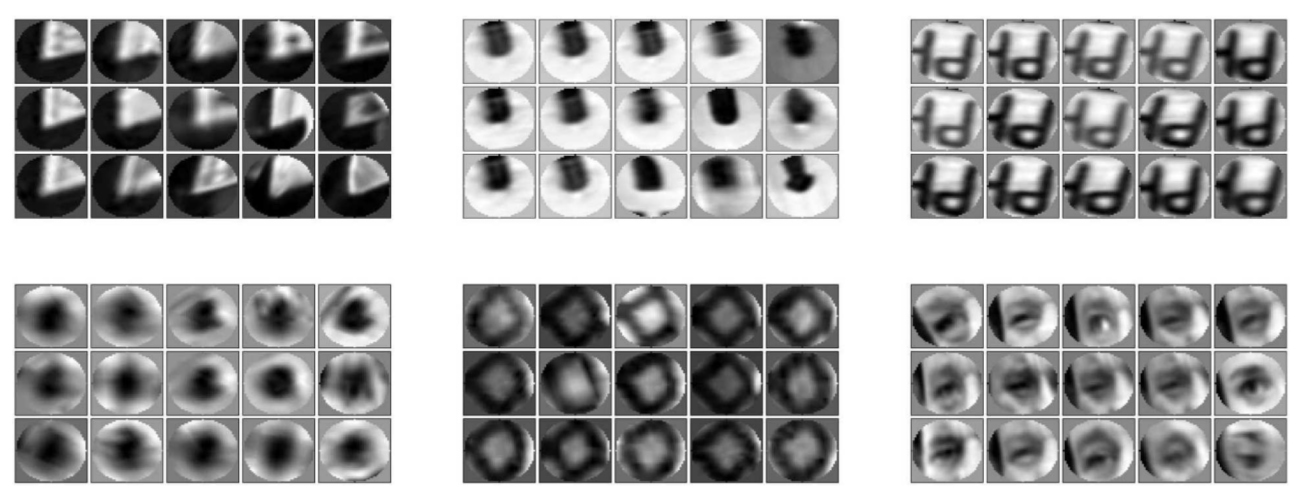
\includegraphics[scale=0.32]{visualWords}
    \else
      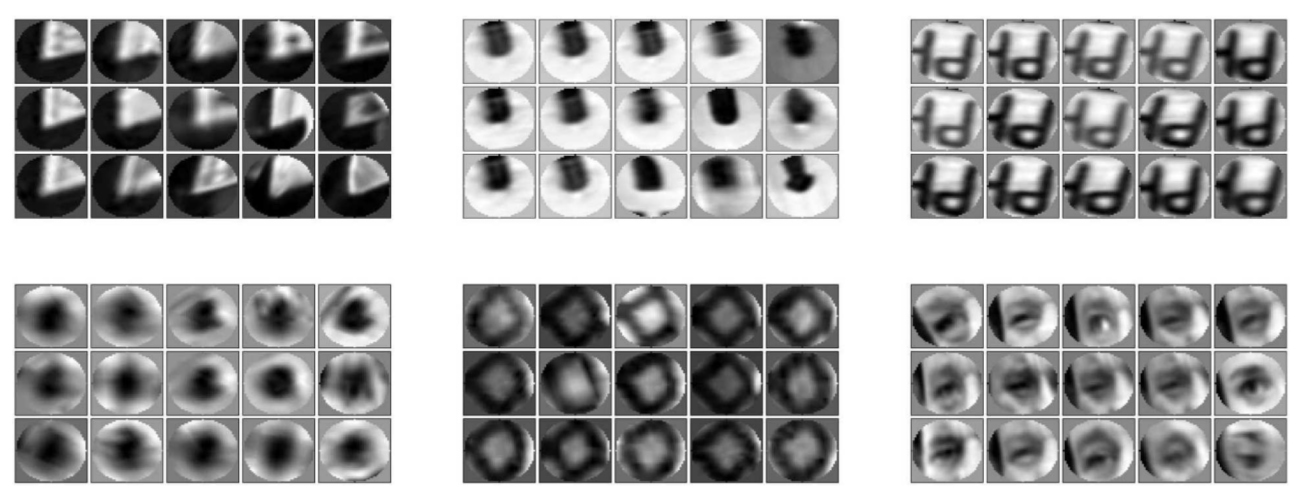
\includegraphics[scale=0.32]{visualWords}
    \fi
    \caption[Các từ trực quan (visual words)]{\textbf{Các từ trực quan (visual words).} Mỗi nhóm là một nhóm các đặc trưng cục bộ được rút trích từ hình ảnh, gom vào cùng một cụm và cùng được biểu diễn bằng một từ trực quan. Hình ảnh được lấy từ bài báo \cite{sivic2009efficient}.}
    \label{FigVisualWords}
  \end{center}
\end{figure}
Có một điều dễ thấy là nếu một hình ảnh được biểu diễn bằng càng nhiều từ trực quan thì hình ảnh đó càng "chi tiết" và độ chính xác của việc so khớp sẽ tăng lên, đồng thời nó cũng khiến cho tốc độ truy vấn nhanh hơn vì các biểu đồ BoW sẽ trở nên "thưa" hơn. Trong thực tế, để truy vấn ảnh trên những tập dữ liệu lớn, để cho kết quả tốt thì số lượng từ trực quan không thể vào khoảng 10,000 từ như trong thí nghiệm của Sivic và Zisserman \cite{sivic2003video} mà phải lên tới hàng triệu từ. Trong khi đó, độ phức tạp của thuật toán k-means là \textit{O(N\textsubscript{w}N\textsubscript{d})} với N\textsubscript{w}, N\textsubscript{d} lần lượt là kích cỡ của từ trực quan và số tập của bộ mô tả huấn luyện (training descriptor set). Trên những tập dữ liệu lớn thì N\textsubscript{d} $\geq$ N\textsubscript{w} nên độ phức tạp luôn lớn hơn $O(N^2_w)$. Do đó ta không thể dùng k-means cho bài toán này. Nister và Stewenius \cite{nister2006scalable} đã đề xuất phương pháp giải quyết cho bài toán này bằng cách xây dựng một cây từ vựng mà về bản chất thì nó chính là thuật toán HKM (Hierarchical K-Means). Để minh họa cho thuật toán này, tác giả đã cho thử nghiệm trên bộ ảnh gồm 1 triệu hình ảnh. Không lâu sau đó, Philbin và các đồng nghiệp \cite{philbin2007object} đã đề xuất một hướng tiếp cận khác dựa trên thuật toán \textit{xấp xỉ k-means}, AKM (Approximate K-Means). Tác giả cũng cho chạy thử nghiệm AKM trên 16.7 triệu đặc trưng để gom cụm thành 1 triệu từ. Các thí nghiệm cho thấy rằng, khi so sánh AKM với k-means thì về độ chính xác thì AKM xấp xỉ k-means tuy nhiên chi phí tính toán chỉ bằng một phần nhỏ của k-means. Còn khi so sánh AKM với HKM thì AKM không những vượt xa về độ chính xác mà còn có thể áp dụng cho những tập dữ liệu lớn. Chi phí tính toán của cả HKM và AKM đều là $O(N_d log(N_w))$.

\section{Sử dụng thông tin không gian ảnh trong truy vấn ảnh}
\label{spatial}

Mặc dù đạt được những kết quả rất đáng chú ý nhưng mô hình cơ bản của BoW vẫn bị giới hạn về độ chính xác do bỏ qua một thông tin quan trọng, đó là thông tin về không gian của các đặc trưng cục bộ. Cấu trúc của mô hình BoW như một cái túi chứa các từ một cách hỗn độn, không theo trật tự nên vị trí của các đặc trưng cục bộ xuất hiện trên hình không được chú ý đến, do đó các đặc trưng cục bộ được xử lý một cách rời rạc, không liên quan tới nhau. Hình \ref{FigExample} minh họa cho việc giảm độ chính xác của mô hình BoW khi không chú ý tới thông tin không gian của các từ trực quan (visual words).

\begin{figure}[!htbp]
  \begin{center}
    \leavevmode
    \ifpdf
      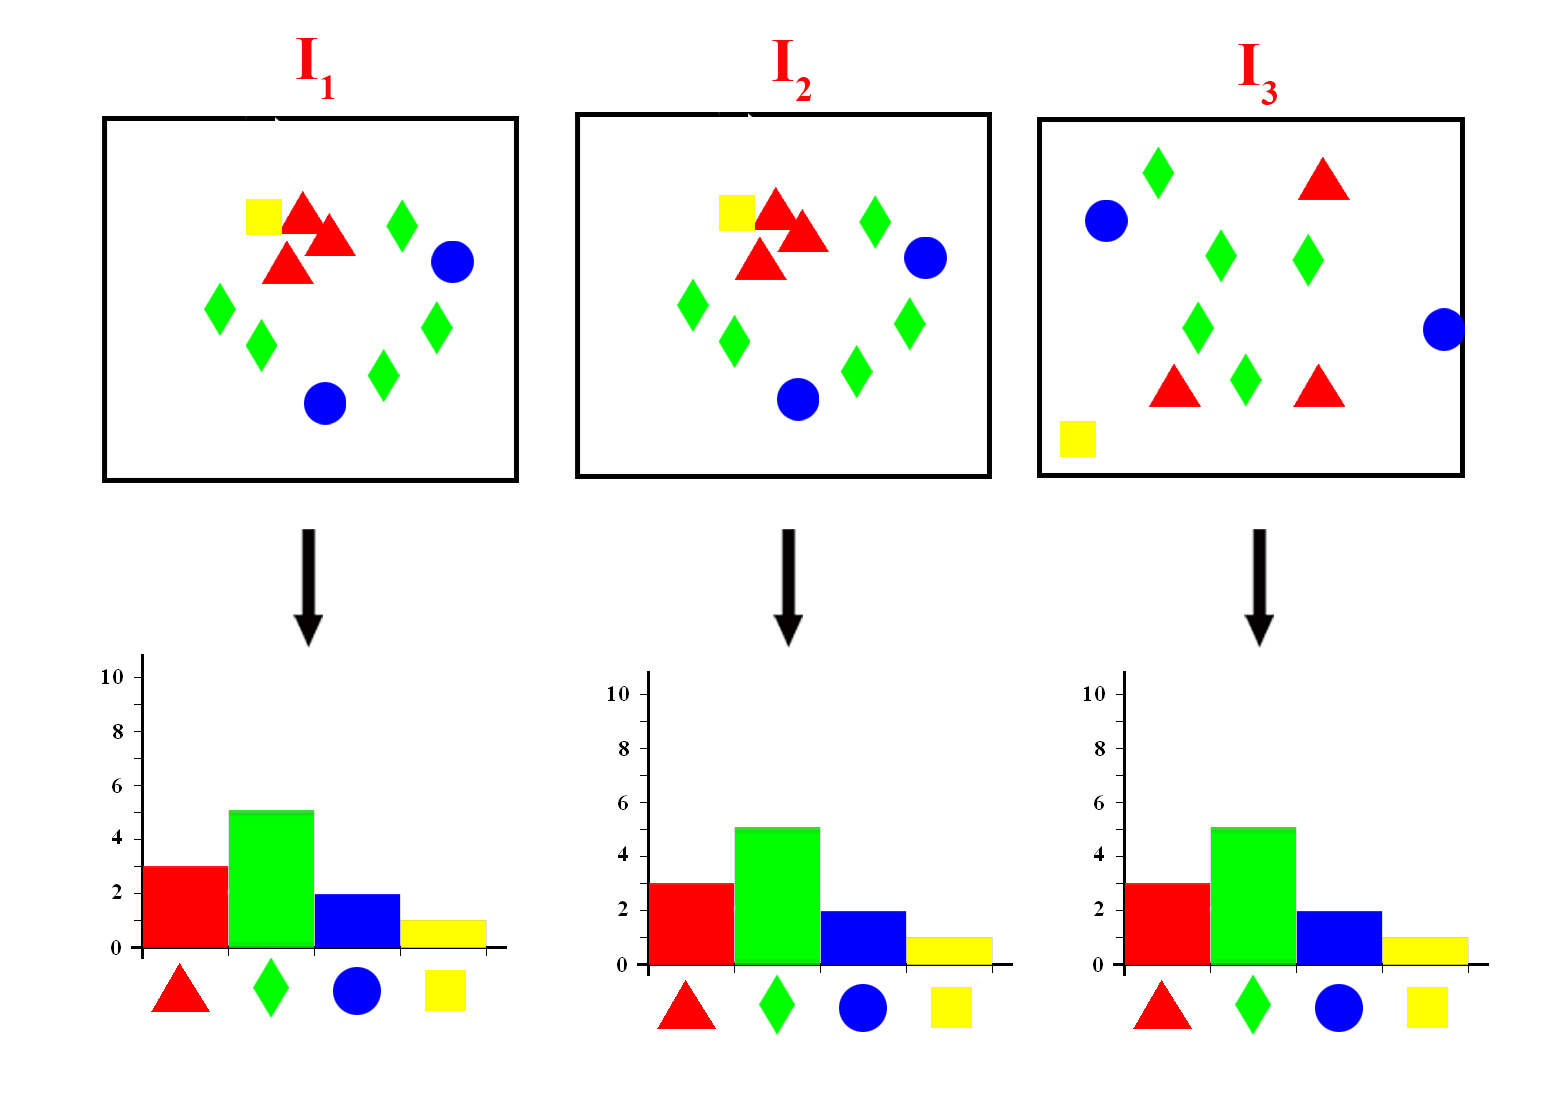
\includegraphics[scale=0.2]{example}
    \else
      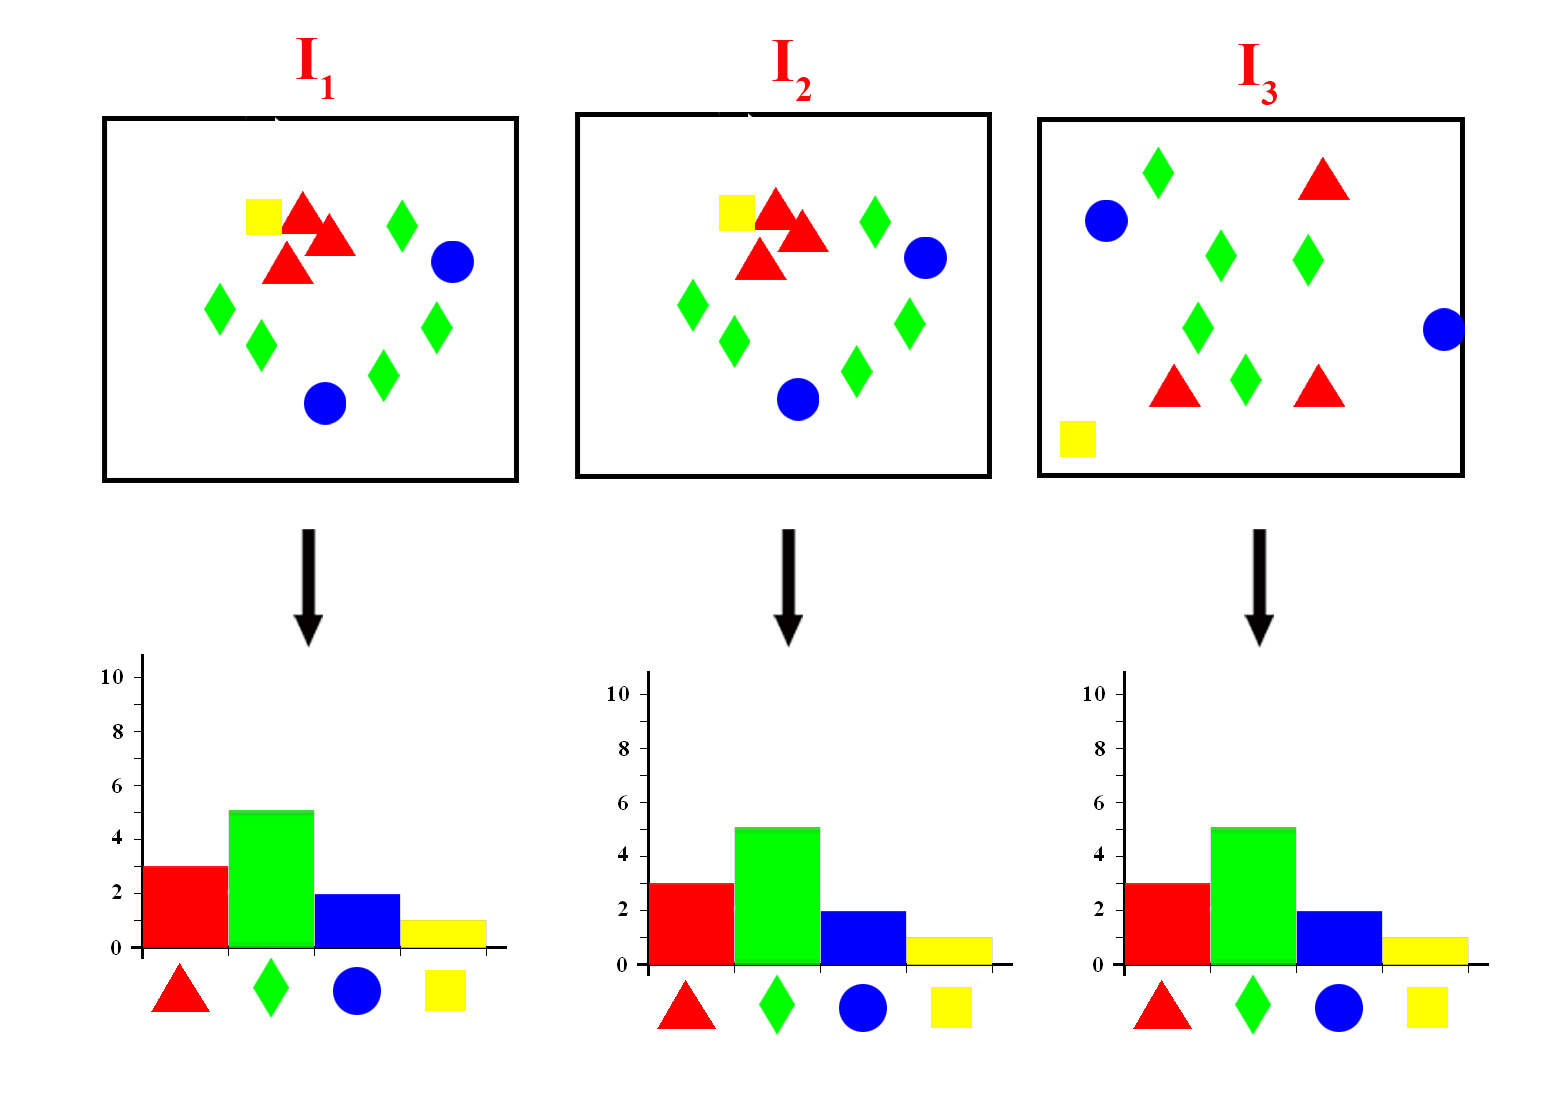
\includegraphics[scale=0.2]{example}
    \fi
    \caption[Bỏ qua thông tin không gian ảnh trong mô hình BoW]{\textbf{Bỏ qua thông tin không gian ảnh trong mô hình BoW.} Nếu bỏ qua thông tin không gian của các từ trực quan, ba hình ảnh trên sẽ được biểu diễn dưới dạng biểu đồ giống nhau do đó chúng sẽ được xem như ba hình ảnh giống nhau. Trong khi đó hình ảnh $I_3$ hoàn toàn khác với $I_1$ và $I_2$.}
    \label{FigExample}
  \end{center}
\end{figure}

Để giải quyết vấn đề trên, rất nhiều công trình nghiên cứu đã được đưa ra. Phần lớn các công trình nghiên cứu được chia ra làm hai dạng là tiếp cận dựa trên đặc trưng hình học và tiếp cận dựa trên thông tin không gian của các đặc trưng cục bộ. Mục \ref{geometry} chúng tôi sẽ trình bày về các phương pháp dựa trên đặc trưng hình học. Còn hướng tiếp cận còn lại sẽ được trình bày chi tiết ở mục \ref{spm}.

\subsection{Các hướng tiếp cận dựa trên đặc trưng hình học}
\label{geometry}
Các phương pháp sử dụng đặc trưng hình học để so khớp thường được dùng ở bước hậu xử lý để nhận dạng hình học. Dưới đây là một vài công trình tiêu biểu sử dụng hướng tiếp cận này.

Sivic và Zisserman \cite{sivic2003video} đã đo đạc sự nhất quán không gian cục bộ (local spatial consistency) trong các so khớp giữa hình ảnh truy vấn và từng hình ảnh trong cơ sở dữ liệu từ đó tái xếp hạng lại danh sách kết quả trả về. Việc đo đạc sự nhất quán không gian cục bộ trong so khớp hình ảnh cũng được đề cập tới trước đó trong các công trình như \cite{zhang1995robust} và \cite{schmid1997local}.

Trong một công trình nghiên cứu \cite{philbin2007object}, tác giả sử dụng thuật toán RANSAC \cite{fischler1981random} để kiểm tra sự nhất quán hình học giữa các đặc trưng cục bộ trùng khớp. RANSAC là một trong những phương pháp phổ biến nhất cho hậu xử lý toàn cục trên hình ảnh. Đặc biệt, trong một công trình khác, Zhang và các đồng nghiệp \cite{zhang2011image} đề xuất mã hóa thông tin không gian ảnh qua các mệnh đề trực quan hình học (GVP) kết hợp với RANSAC đã cho kết quả rất đáng chú ý với bộ dữ liệu lên tới hàng triệu ảnh.

Trong khi đó, công trình \cite{lin2010local} và \cite{lampert2009detecting} lại xếp hạng các hình ảnh dựa trên điểm số so khớp của hình ảnh truy vấn với những cửa sổ con được định vị trên hình. Phương pháp này mã hóa được nhiều thông tin không gian ảnh hơn so với môt hình BoW trên toàn bộ tấm hình và giúp định vị hình ảnh truy vấn.

Nhìn chung, những phương pháp sử dụng hướng tiếp cận hình học đều cho kết quả tốt. Tuy nhiên, khi vùng truy vấn lớn hơn thì chúng chỉ được dùng để tái xếp hạng một số lượng giới hạn ở các hình ảnh ở top đầu của kết quả trả về vì vấn đề về chi phí cho bộ nhớ và tốc độ thực hiện.

\subsection{Các hướng tiếp cận dựa trên thông tin không gian của các đặc trưng cục bộ}
\label{spm}

Hướng tiếp cận dựa trên đặc trưng hình học là hướng tiếp cận mang tính toàn cục, tức là xem xét đối tượng dưới một cái nhìn tổng quan, toàn thể chứ không xem xét chi tiết những thành phần cấu thành nó. Hướng tiếp cận dựa trên các đặc trưng cục bộ lại ngược lại, xem đối tượng là một tập hợp của nhiều thành phần và dựa trên những thành phần đó để xác định đối tượng. Lazebnik \cite{lazebnik2006beyond} đã giới thiệu một phương pháp nền tảng, được bắt nguồn từ ý tưởng \textit{so khớp phân cấp} (pyramid matching) của Grauman và Darrell \cite{grauman2005pyramid}, đó là phương pháp \textit{so khớp không gian phân cấp} (Spatial Pyramid Matching - SPM). Ý tưởng của phương pháp này là lặp đi lặp lại việc chia nhỏ hình ảnh và tính toán biểu đồ của các đặc trưng cục bộ với mức độ chi tiết tăng dần. SPM đã giúp nâng cao một cách đáng kể độ chính xác cho mô hình BoW và tỏ ra là một phương pháp đơn giản nhưng hiệu quả. Mặc dù vậy, SPM cũng làm tăng thời gian thực hiện truy vấn bởi khi mức độ chi tiết càng cao thì kích cỡ biểu đồ của các đặc trưng cục bộ cũng tăng theo làm tăng chi phí tính toán trong quá trình so khớp, vì vậy SPM vẫn chưa thích hợp cho các bài toán yêu cầu thời gian thực.

\section{Kết chương}

Việc biểu diễn hình ảnh bằng các đặc trưng cục bộ đã đặt nền tảng cho việc đưa ra các phương pháp để truy vấn đối tượng trên ảnh. Mô hình BoW đã chứng minh tính hiệu quả của mình trong truy vấn ảnh và việc kết hợp phương pháp chỉ mục ngược (inverted index) giúp giảm đáng kể thời gian thực hiện truy vấn. Tuy nhiên, mô hình BoW vẫn bị giới hạn về độ chính xác do bỏ qua thông tin không gian ảnh. Trong khi đó, rất nhiều hướng tiếp cận khác tận dụng được thông tin này đã nâng độ chính xác của truy vấn lên rất nhiều nhưng lại không quan tâm nhiều tới thời gian thực hiện.

Phương pháp chúng tôi đề xuất tập trung vào cả độ chính xác và thời gian truy vấn. Để đạt được mục đích đó, chi phí bộ nhớ cao có thể được chấp nhận.


\chapter{Phương pháp đề xuất}
\label{chapter:proposed}
\ifpdf
    \graphicspath{{Chapter3/Chapter3Figs/PNG/}{Chapter3/Chapter3Figs/PDF/}{Chapter3/Chapter3Figs/}}
\else
    \graphicspath{{Chapter3/Chapter3Figs/EPS/}{Chapter3/Chapter3Figs/}}
\fi

\markboth{\MakeUppercase{\thechapter. Tích hợp thông tin không gian ảnh vào chỉ mục ngược}}{\thechapter. Tích hợp thông tin không gian ảnh vào chỉ mục ngược}

Rất nhiều công trình được đưa ra để giải quyết bài toán truy vấn ảnh (mục \ref{local-features} và \ref{bag-of-words}). Phương pháp cơ bản để giải quyết bài toán là biểu diễn một hình ảnh dưới dạng mô hình Bag-of-visual-Words (BoW), sau đó xếp hạng các hình ảnh sử dụng phương pháp tf-idf và dùng chỉ mục ngược (inverted index) để tăng hiệu suất tính toán. Tuy nhiên, phương pháp trên vẫn còn bị giới hạn về độ chính xác do chưa sử dụng đến thông tin không gian ảnh. Các phương pháp được đưa ra trong những năm gần đây để giải quyết vấn đề này đã được giới thiệu trong mục \ref{spatial}.\\

Trong chương này, chúng tôi sẽ mô tả phương pháp đề xuất để tích hợp thông tin không gian ảnh vào chỉ mục ngược. Trước tiên chúng tôi sẽ nhắc lại những công trình khơi nguồn ý tưởng cho phương pháp của chúng tôi. Sau đó là phần trình bày chi tiết phương pháp đề xuất và những cải tiến nhằm nâng cao hiệu suất cho hệ thống.

\section{Chỉ mục ngược với biểu diễn Bag-of-Visual-Words}
\label{sec:inverted-index}
Như đã được giới thiệu sơ lược trọng mục 2.2.1, chỉ mục ngược (inverted index) là phương pháp phổ dùng để tối ưu hóa tốc độ truy vấn cơ sở dữ liệu bằng việc lưu trữ trước một ánh xạ từ nội dung đến vị trí trong cơ sở dữ liêu. Nói cách khác, chỉ mục ngược là một cấu trúc dữ liệu chủ yếu bao gồm 2 trường là khóa và giá trị. Mỗi khóa đại diện cho một \textit{từ}, và phần giá trị của tương ứng lưu trữ danh sách các văn bản có chứa từ đó. Vì vậy ta có thể dễ dàng lấy được danh sách tất cả các văn bản chứa từ truy vấn.

Chính vì sự thành công của các kỹ thuật tìm kiếm văn bản, chỉ mục ngược đã được mở rộng để sử dụng cho tìm kiếm ảnh trên cơ sở dữ liệu lớn. Để có thể xây dựng chỉ mục ngược cho cơ sở dữ liệu ảnh, mô hình BoW đã được sử dụng để biểu diễn hình ảnh. Quá trình xây dựng chỉ mục ngược như sau: (i) một bộ dò tìm các đặc trưng sẽ phát hiện những điểm quan trọng, sau đó một bộ mô tả sẽ trích rút trích được những đặc trưng xung quanh điểm đó; (ii) các đặc trưng được gom thành các cụm để tạo thành từ điển, mỗi cụm là một tập các đặc trưng gần giống nhau và trung tâm của mỗi cụm là một visual word, mỗi visual word sẽ được gán một mã số khác nhau; (iii) Trường giá trị trong tệp chỉ mục ngược sẽ lưu trữ danh sách các hình ảnh có chứa các visual word tương ứng. Quá trình tạo tập chỉ mục ngược (inverted file) được minh họa trong Hình \ref{FigInvertedFile}.

\begin{figure}[!htbp]
  \begin{center}
    \leavevmode
    \ifpdf
      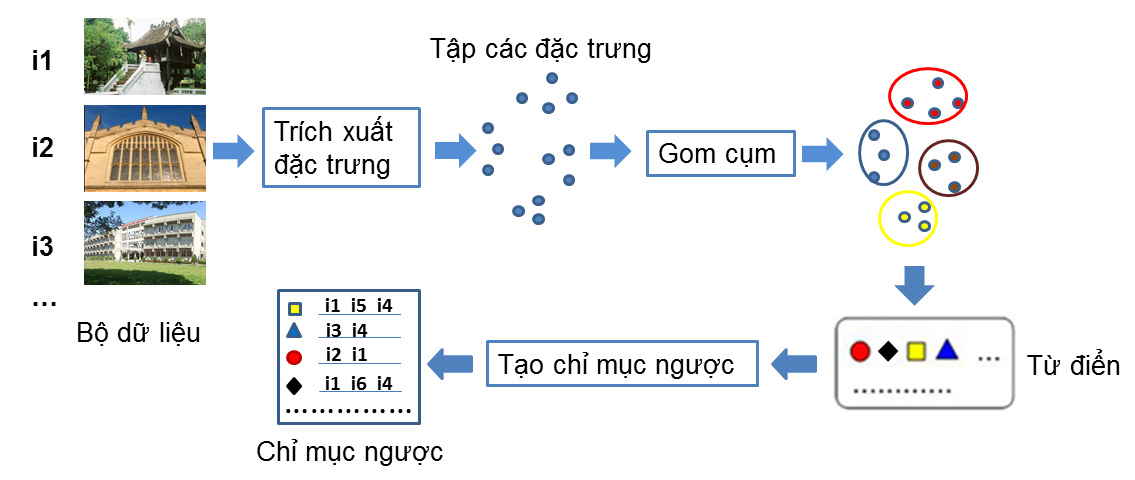
\includegraphics[scale=0.51]{invertedFile}
    \else
      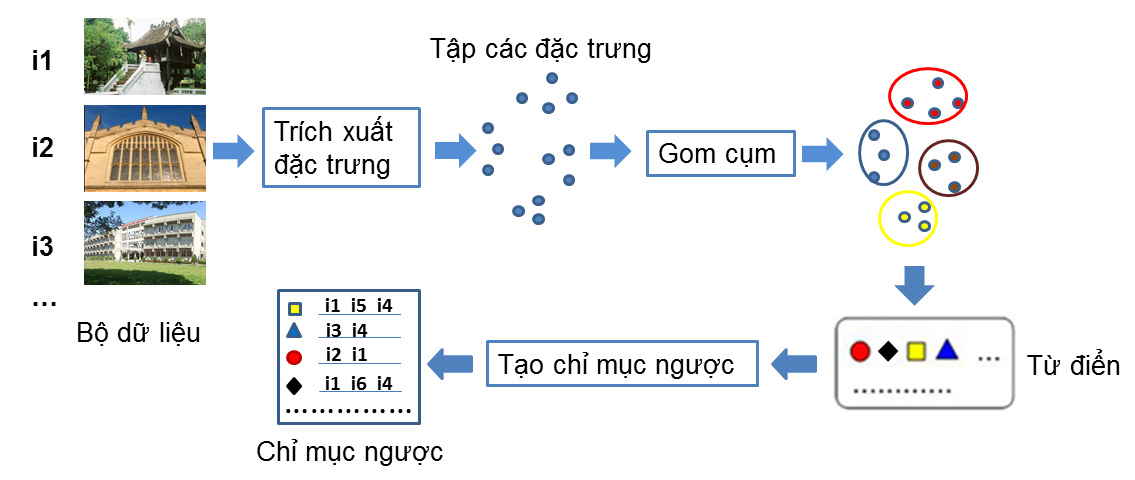
\includegraphics[scale=0.51]{invertedFile}
    \fi
    \caption[Quá trình tạo tập chỉ mục ngược]{Quá trình tạo tập chỉ mục ngược (inverted index file).}
    \label{FigInvertedFile}
  \end{center}
\end{figure}

Trong quá trình truy vấn, các đặc trưng sẽ được rút trích từ hình ảnh truy vấn, sau đó từ các đặc trưng ta sẽ lấy được các visual word bằng cách sử dụng từ điển sau đó tra cứu trong tập chỉ mục ngược để lấy được các hình ảnh ứng viên. Những hình ảnh nào có số lượng visual word trùng với các visual word trong hình ảnh truy vấn càng nhiều thì sẽ càng được xếp hạng cao hơn trong danh sách kết quả truy vấn trả về. Kỹ thuật này được gọi là \textit{bầu chọn} (voting).

Bên cạnh kỹ thuật bầu chọn, để nâng cao độ chính xác của kết quả trả về, người ta có thể thêm một bước tái xếp hạng danh sách kết quả bằng cách tính khoảng cách trong không gian đặc trưng giữa hình ảnh truy vấn và các hình ảnh ứng viên sử dụng biểu diễn BoW của chúng. Tuy nhiên, chi phí tính toán của quá trình này rất cao dẫn đến thời gian thực hiện truy vấn tăng đáng kể.\\

Trong thí nghiệm được trình bày ở Chương 4, chúng tôi sẽ so sánh cả hai phương pháp bầu chọn và tái xếp hạng với phương pháp được đề xuất.\\

\section{Tích hợp thông tin không gian ảnh vào chỉ mục ngược}
\label{sec:intergrated}
Phương pháp chúng tôi đề xuất nhằm tích hợp thông tin không gian ảnh vào chỉ mục ngược được bắt nguồn từ ý tưởng của một công trình nghiên cứu của Lazebnik và các đồng nghiệp \cite{lazebnik2006beyond}. Trong công trình đó, thay vì sử dụng một biểu đồ (histogram) chung  của các visual word để biểu diễn một hình ảnh thì họ chia hình ảnh thành các nhiều phần sử dụng lưới ô vuông phân cấp (hay còn được gọi là không gian phân cấp - spatial pyramid). Một lưới ô vuông tại cấp \textit{l} sẽ chia hình ảnh thành $2^l \times 2^l$ ô với kích cỡ như nhau. Do đó, số ô vuông trên lưới ở cấp 0 là $1 \times 1$; cấp 1 là $2 \times 2$. Nếu cấp \textit{l} càng cao thì lưới ô vuông sẽ càng dày đặc hơn. Nếu coi mỗi ô của hình ảnh được chia bởi lưới ô vuông phân cấp là một hình ảnh độc lập, dựa trên mô hình BoW ta sẽ tính được các biểu đồ độc lập. Chính vì mức độ chia tiết của các biểu đồ khác nhau nên chúng sẽ được đánh trọng số khác rồi rồi được ghép nối với nhau để tạo thành một vector đặc trưng biểu diễn cho hình ảnh. Bằng cách biểu diễn như vậy, các hình ảnh có sự phân bố các visual word tương tự nhau sẽ được biễu diễn bằng những biểu đồ ghép nối gần giống nhau.

Dựa trên ý tưởng của nghiên cứu trên, chúng tôi đề xuất sử dụng không gian phân cấp để tăng cường mức độ bầu chọn và lập chỉ mục của kỹ thuật đánh chỉ mục ngược căn bản. Ý tưởng được chúng tôi đưa ra là chia hình ảnh thành nhiều ô sử dụng không gian phân cấp và giới hạn ở một cấp xác định. Sau đó các visual word sẽ được đánh số tương ứng với các ô chúng rơi vào. Ta sẽ duyệt qua tất cả các ô ở tất cả các cấp khác nhau để thực hiện việc bầu chọn. Do đó, nếu hai hình ảnh chứa các visual word giống nhau trong cùng một ô sẽ nhận được nhiều lượt bầu chọn hơn so với hai hình ảnh có các visual word giống nhau nhưng lại nằm rải rác ở các ô khác nhau. Các lượt bầu chọn sẽ được đánh trọng số tùy theo từng cấp. Nếu cấp càng cao hay diện tích của mỗi ô càng hẹp thì trọng số của lượt bầu chọn càng cao. Trọng số tại cấp \textit{l} sẽ là $\frac{1}{2^{L-l}}$.

Một trong những điểm đặc biệt của phương pháp đề xuất là chúng tôi sử dụng đa chỉ mục ngược. Tức là chia thành nhiều tập chỉ mục ngược khác nhau nhưng các tập vẫn giữ được cấu trúc căn bản của chỉ mục ngược. Mỗi tập sẽ dùng để lưu trữ chỉ muc cho một ô trên không gian phân cấp. Nếu cấp độ cao nhất của không gian phân cấp là \textit{L} thì tổng số lượng tập chỉ mục ngược sẽ là $\frac{1}{3}(4^{L+1} - 1)$ và mỗi cấp độ sẽ có $2^l \times 2^l$ tập chỉ mục ngược với $0 \leq l \leq L$. Hình \ref{FigBasicIdea} mô tả khái quát cho phương pháp được đề xuất.

\begin{figure}[!htbp]
  \begin{center}
    \leavevmode
    \ifpdf
      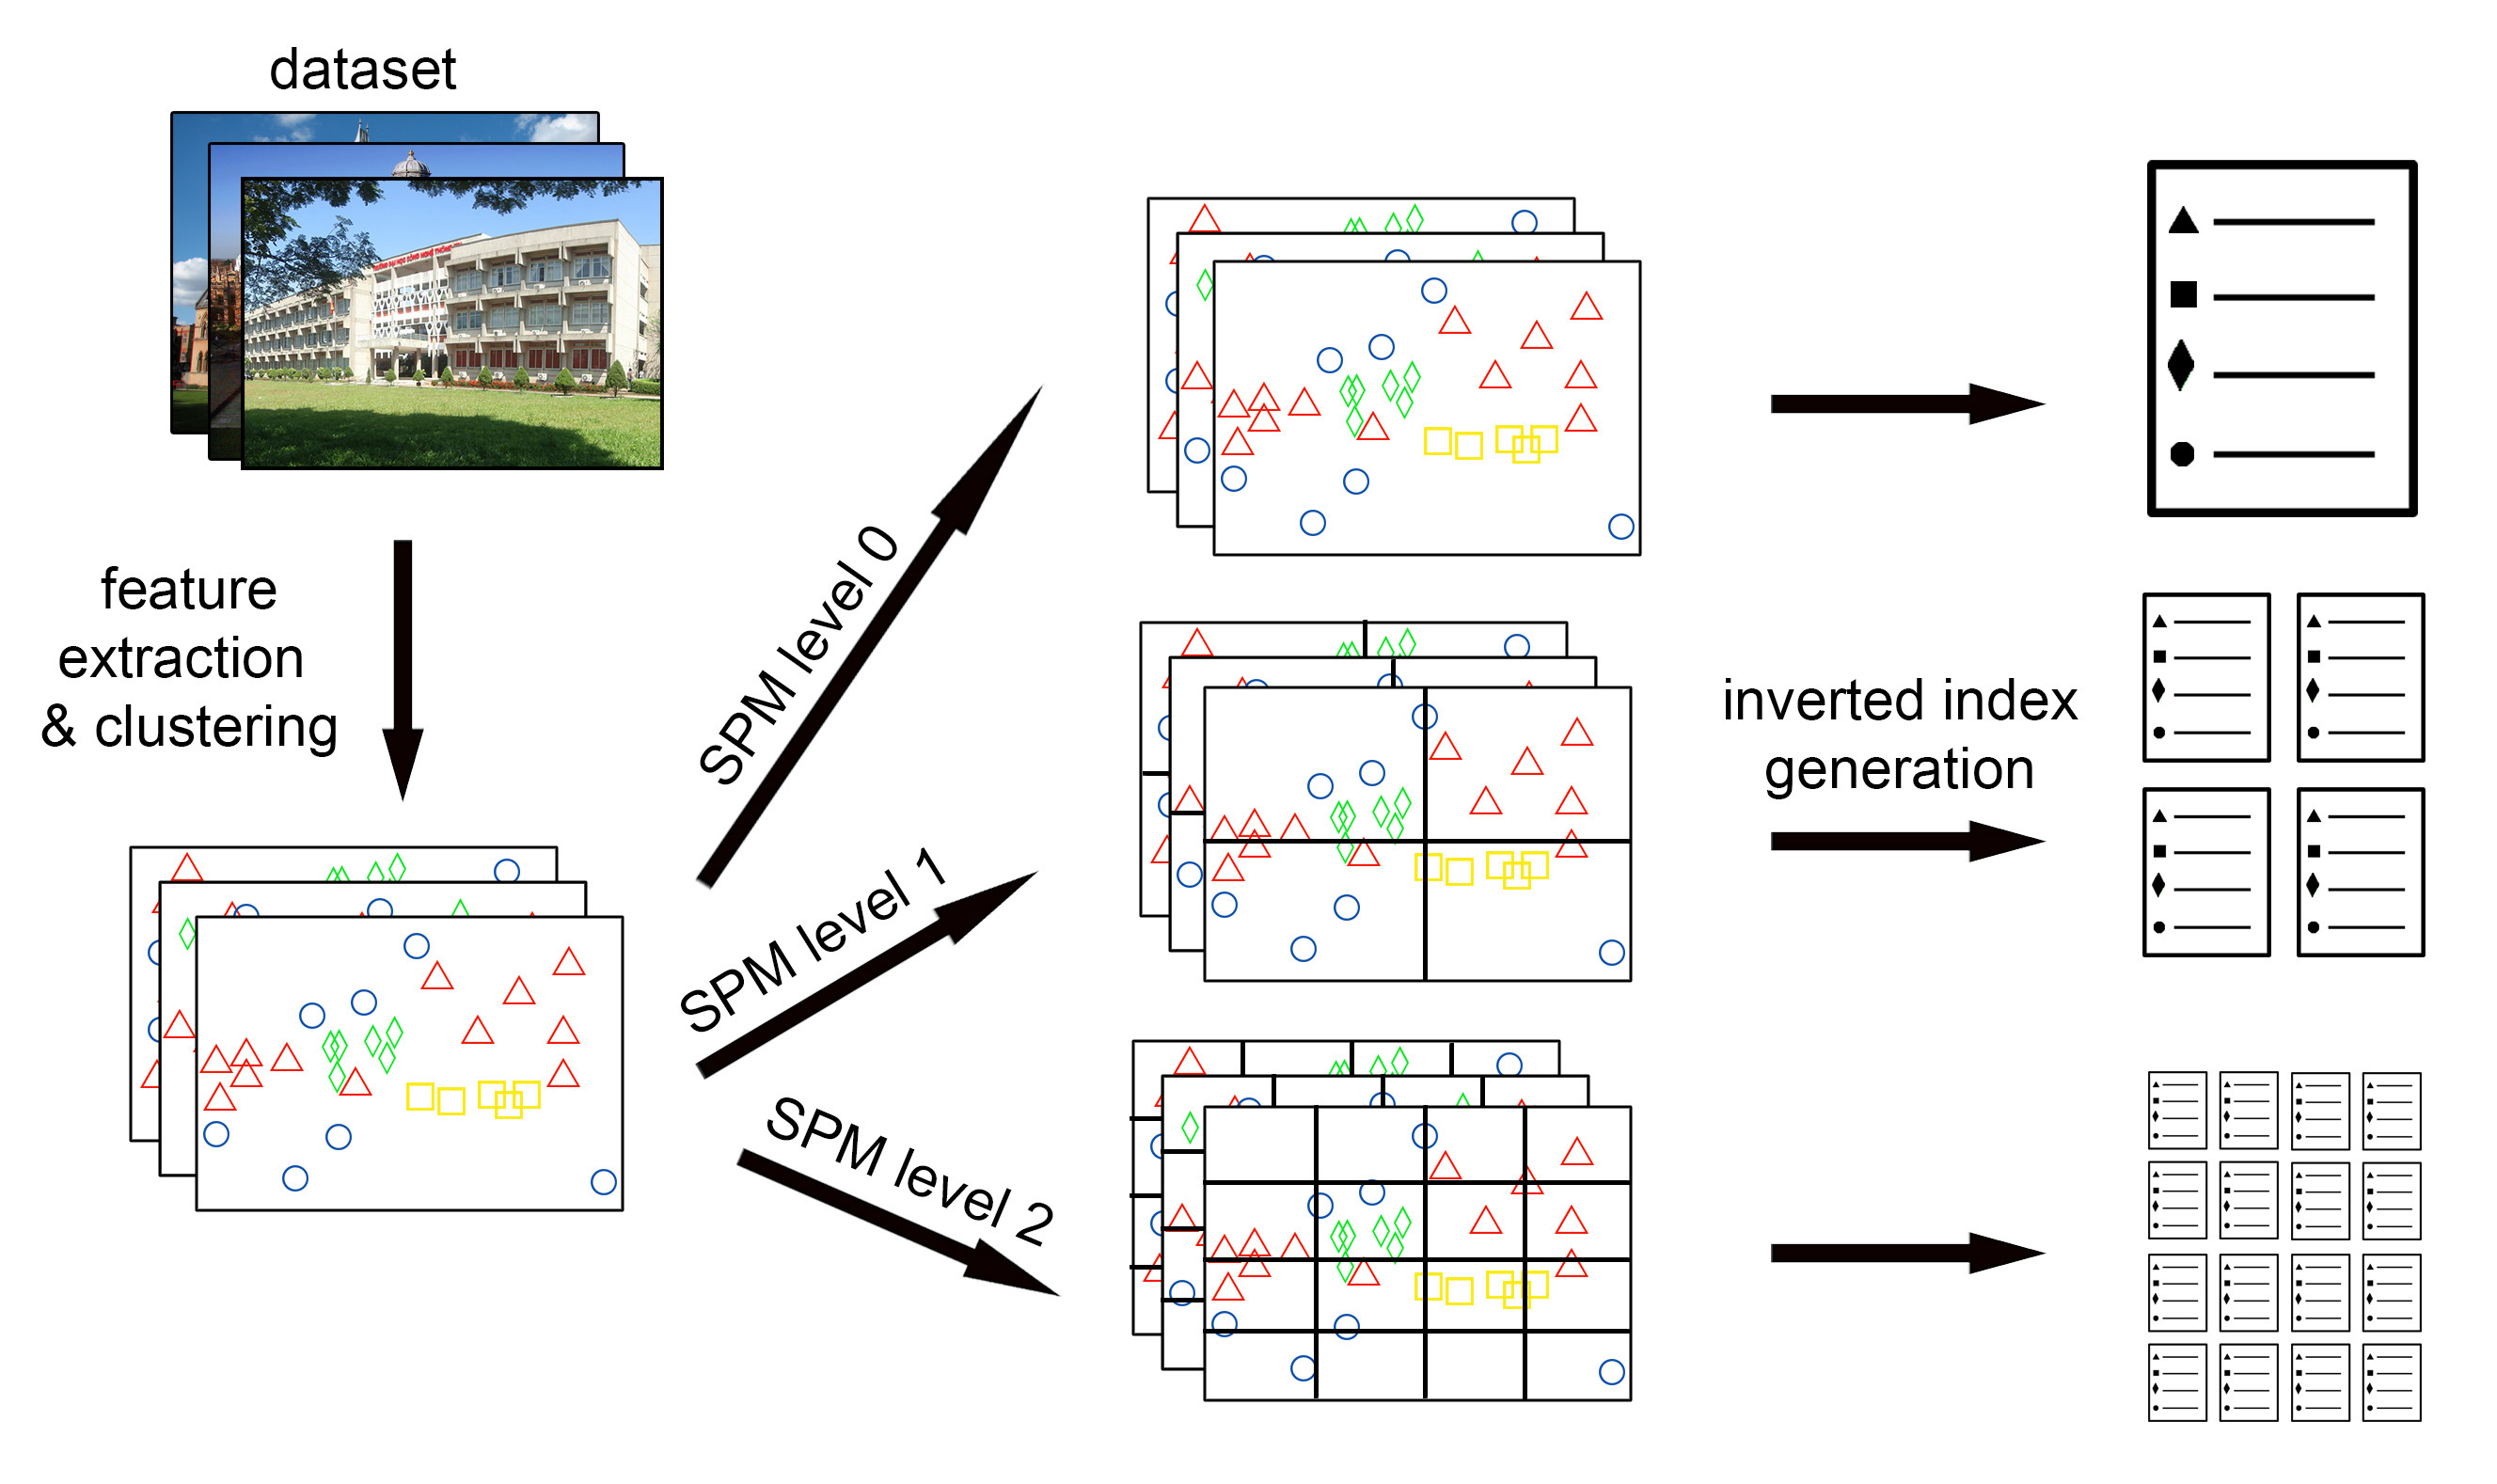
\includegraphics[scale=0.15]{basicIdea}
    \else
      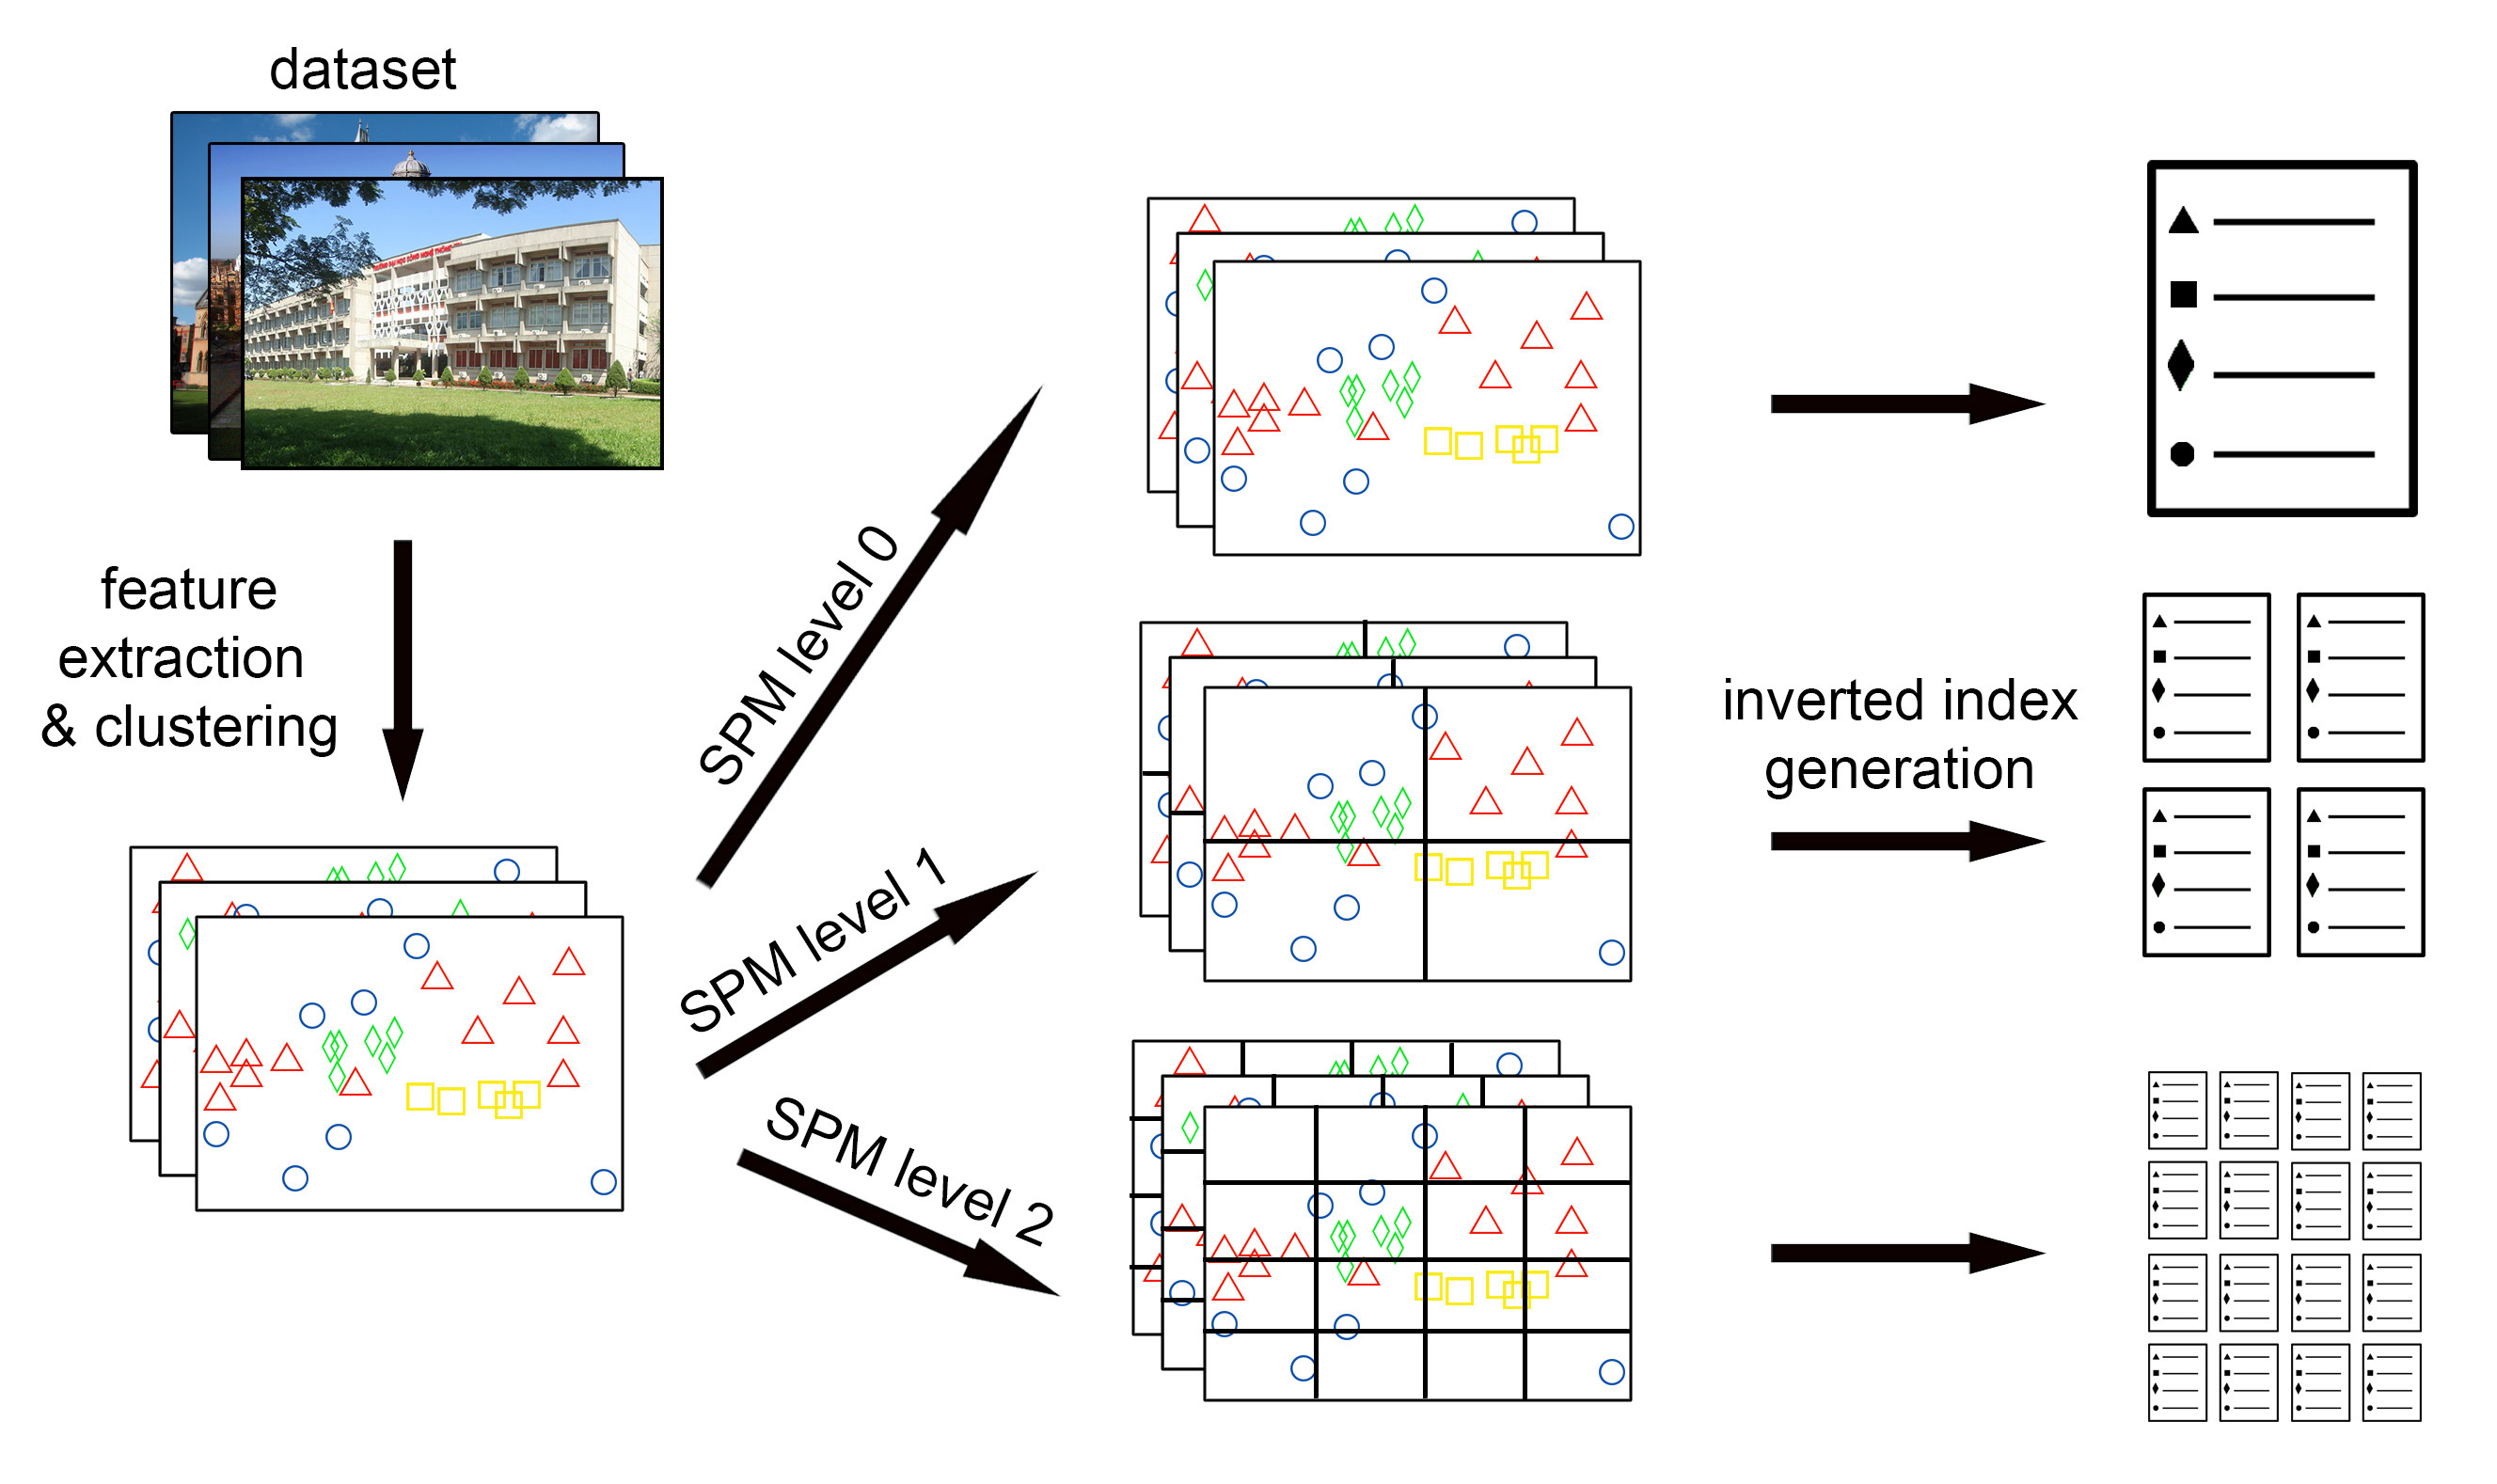
\includegraphics[scale=0.15]{basicIdea}
    \fi
    \caption[Khái quát về phương pháp đề xuất]{Khái quát về phương pháp đề xuất.}
    \label{FigBasicIdea}
  \end{center}
\end{figure}

Khi thực hiện quá trình rút trích các đặc trưng cho tất cả các hình trong cơ sở dữ liệu, thông tin không gian của các đặc trưng đó sẽ được lưu trữ lại. Sau đó các bộ mô tả (descriptors) của đặc trưng (ví dụ như key points) sẽ được lượng tử hóa để tạo thành một bảng từ vựng của các visual word (từ điển). Mỗi hình ảnh sẽ chứa một tập các visual word. Tiếp đó ta sẽ sử dụng không gian phân cấp để chia tất cả các hình ảnh thành các ô nhỏ với "độ mịn" tăng dần dựa trên cấp được định nghĩa. Lúc này, thông tin không gian của các đặc trưng đã được lưu trước đó sẽ được sử dụng để xác định xem visual word đó có thuộc ô đang xét hay không. Tất cả các visual word được tìm thấy trong mỗi ô sẽ được thu thập lại. Tiếp theo, tập hợp của các visual word được tìm thấy trong mỗi ô của các hình ảnh sẽ được dùng để sinh ra một tập chỉ mục ngược tương ứng với ô đó. Số lượng tập chỉ mục ngược được sinh ra bằng với tổng số ô của không gian phân cấp.

Trong quá trình truy vấn, các đặc trưng cũng được rút trích từ hình ảnh truy vấn. Sau đó chúng được đưa vào từ điển để lấy được các visual word tương ứng. Dựa vào vị trí của các visual word này, ta có thể xác định được chúng thuộc ô nào tại mỗi cấp của mô hình không gian phân cấp. Từ đó ta có thể có thể truy xuất ngay lập tức tới tập chỉ mục ngược tương ứng với mỗi ô để lấy và xếp hạng danh sách hình ảnh ứng viên một cách đồng thời. Ta xếp hạng hình ảnh bằng phương pháp bầu chọn nên việc bầu chọn diễn ra trong mỗi lần truy xuất tập chỉ mục ngược, do đó danh sách đếm số lượt bầu chọn sẽ được cập nhật liên tục trong suốt quá trình truy xuất các tập chỉ mục ngược. Khi quá trình bầu chọn kết thúc, ta sẽ tổng hợp toàn bộ số lượt bầu chọn cho từng hình rồi xếp hạng các hình theo số lượt bầu chọn. Toàn bộ quá trình truy vấn của phương pháp đề xuất được minh họa trong Hình \ref{FigQueryProcess}.

\begin{figure}[!htbp]
  \begin{center}
    \leavevmode
    \ifpdf
      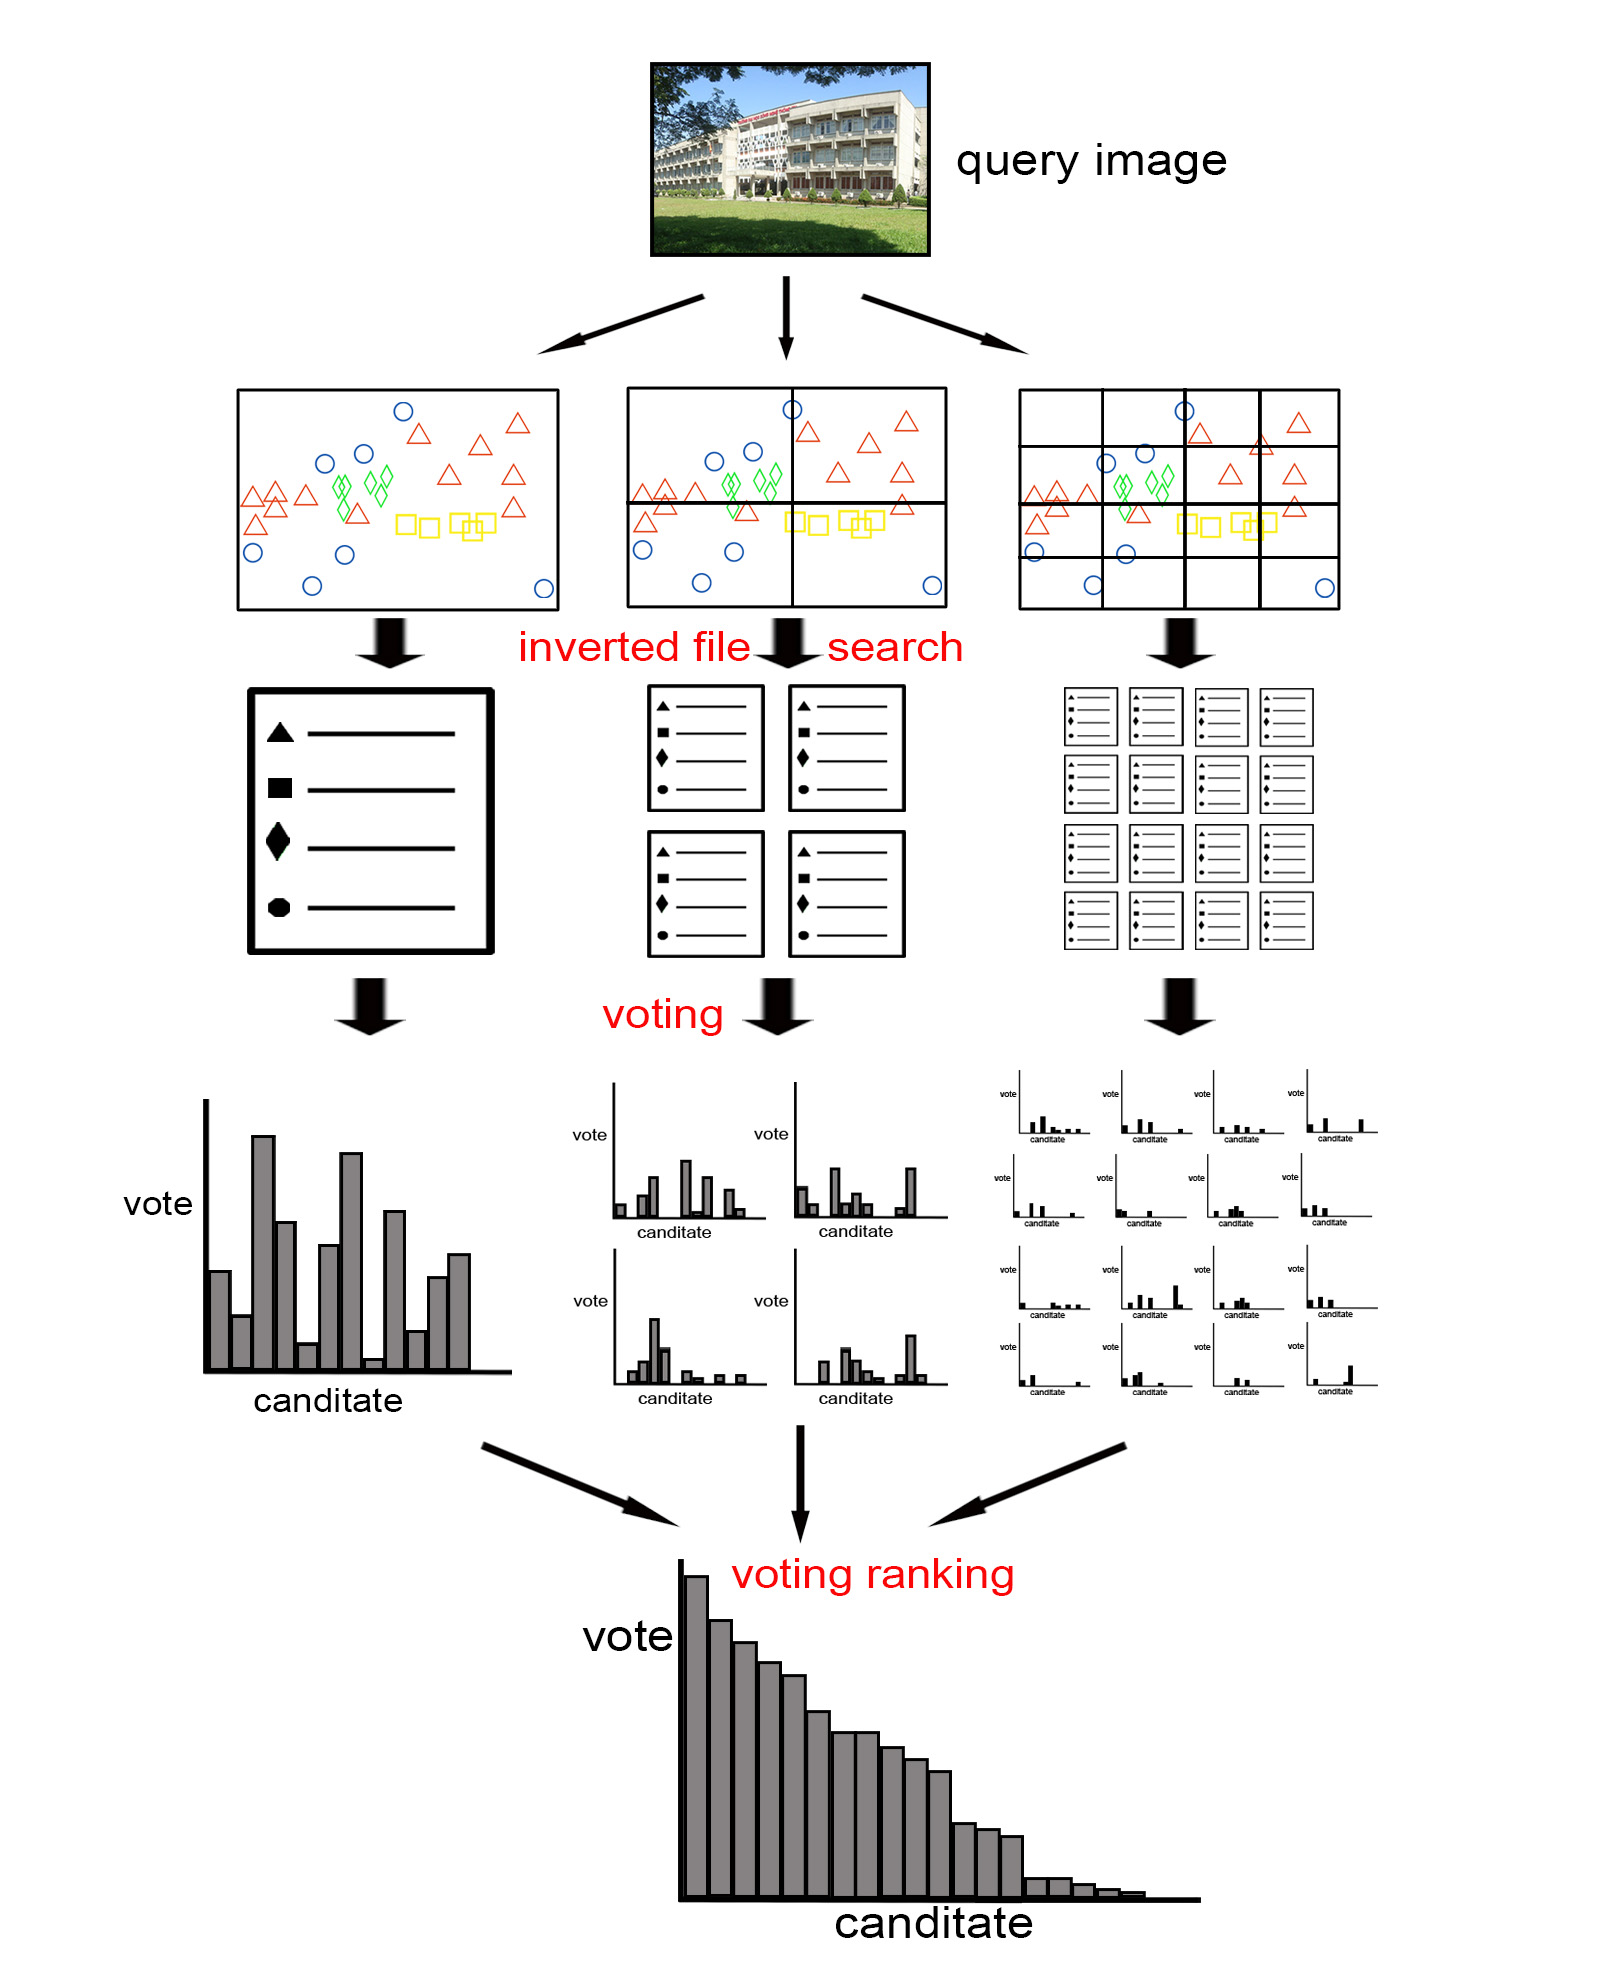
\includegraphics[scale=0.25]{queryProcess}
    \else
      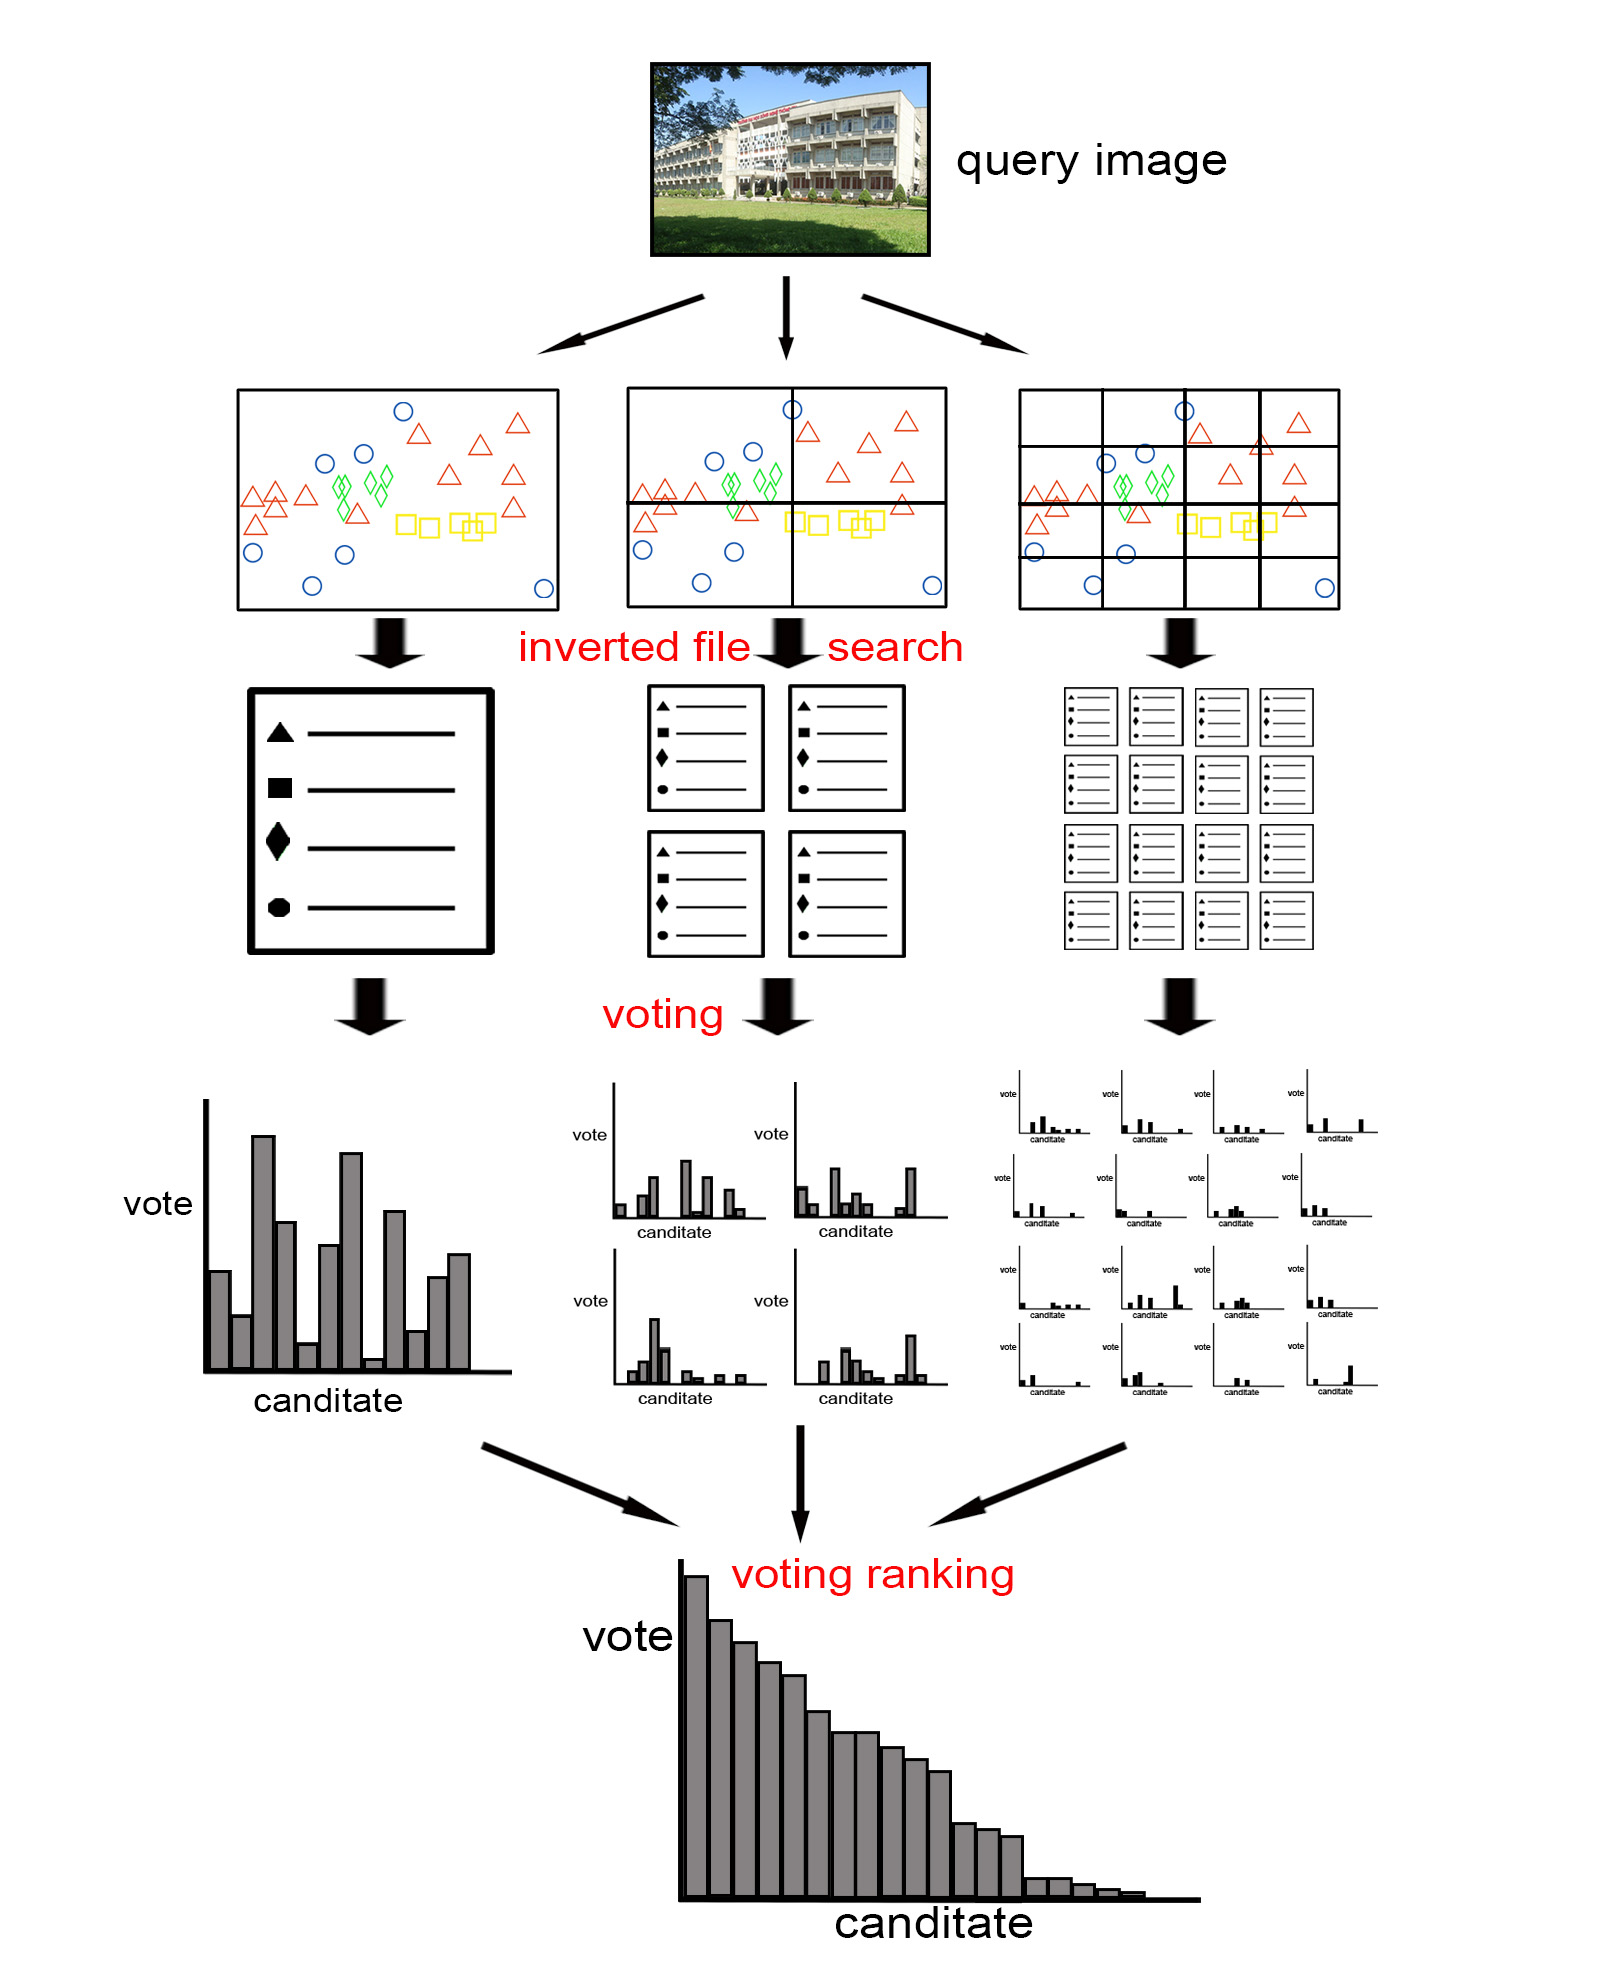
\includegraphics[scale=0.25]{queryProcess}
    \fi
    \caption[Quá trình truy vấn của phương pháp đề xuất]{Quá trình truy vấn của phương pháp đề xuất.}
    \label{FigQueryProcess}
  \end{center}
\end{figure}

\chapter{Tích hợp thông tin không gian ảnh vào inverted index}
\ifpdf
    \graphicspath{{Chapter3/Chapter3Figs/PNG/}{Chapter3/Chapter3Figs/PDF/}{Chapter3/Chapter3Figs/}}
\else
    \graphicspath{{Chapter3/Chapter3Figs/EPS/}{Chapter3/Chapter3Figs/}}
\fi

\section{Ý tưởng phương pháp}
\markboth{\MakeUppercase{\thechapter. My Third Chapter }}{\thechapter. My Third Chapter}
Lorem ipsum dolor sit amet, consectetur adipiscing elit. Pellentesque et semper arcu. In augue eros, varius ac aliquam vel, suscipit vitae erat. Curabitur sodales semper lectus, eu imperdiet quam vulputate quis. Sed consectetur scelerisque rhoncus. Cras sed pretium augue. Pellentesque magna eros, mattis sed massa nec, pellentesque gravida eros. Sed nec tellus vel urna pharetra feugiat. Fusce ultricies tincidunt facilisis. Suspendisse sodales est metus, quis tincidunt dolor molestie ut. Etiam vitae dignissim mi. Suspendisse pulvinar tellus ac libero rutrum, quis sagittis ligula rhoncus.

Nam id lectus quis ligula ullamcorper pharetra. In eget commodo sem. Curabitur dictum imperdiet urna, vitae euismod lorem tristique pellentesque. Proin sollicitudin elementum lobortis. Curabitur posuere, arcu suscipit porta consectetur, nisi urna faucibus mauris, in elementum risus dolor at diam. Nunc fermentum lobortis imperdiet. Cras pellentesque elementum rutrum. In hac habitasse platea dictumst. Quisque elementum felis eu risus venenatis congue. Nullam ornare, justo sed pulvinar semper, risus elit ullamcorper libero, viverra euismod metus diam quis urna. Suspendisse neque quam, condimentum sit amet consectetur malesuada, vehicula fringilla augue. Etiam eu mi commodo, egestas tellus et, dapibus tellus. Cras nec urna justo.

\section{Cài đặt thí nghiệm}
Lorem ipsum dolor sit amet, consectetur adipiscing elit. Vestibulum euismod libero a augue suscipit, a dignissim justo ullamcorper. Nunc in tincidunt dolor, sed feugiat ante. Curabitur ut elit sit amet dui euismod congue porttitor rhoncus enim. Donec in mollis massa, et sagittis est. Duis est dui, suscipit id sollicitudin vel, malesuada non metus. Vivamus tincidunt libero non nunc dignissim, interdum auctor lorem lacinia. Praesent ultrices nec turpis placerat consectetur. Maecenas volutpat lobortis interdum. Fusce ullamcorper nunc at varius bibendum. Praesent at ipsum sagittis, facilisis leo ac, commodo orci.

Proin eu velit semper, molestie ipsum sit amet, consequat quam. Fusce rhoncus est in facilisis mattis. Pellentesque habitant morbi tristique senectus et netus et malesuada fames ac turpis egestas. Vivamus accumsan, erat sed egestas luctus, orci turpis posuere dolor, ut tempor magna enim et mauris. Maecenas in scelerisque quam, id bibendum lacus. Nullam rutrum odio id magna porttitor tincidunt. Cum sociis natoque penatibus et magnis dis parturient montes, nascetur ridiculus mus. Aliquam feugiat elit sapien, eget consectetur sapien tempor et. Aenean tempus eleifend laoreet. Vivamus nec mollis orci. Maecenas sit amet quam nibh. Phasellus blandit fringilla massa faucibus porta. Fusce mattis pellentesque leo, sed auctor mi lobortis viverra. Donec sed arcu non orci gravida accumsan nec in diam. Proin malesuada enim sed est sagittis, tincidunt sollicitudin metus suscipit. Vivamus dapibus suscipit diam, fringilla fermentum arcu dignissim eu.

Aliquam eget velit vitae ligula pharetra malesuada. Maecenas ut facilisis lorem, in dapibus dolor. Curabitur pulvinar dolor a adipiscing dignissim. Maecenas sed porttitor ligula. Morbi vitae lacus laoreet, posuere odio eget, vehicula dui. Pellentesque lectus metus, rutrum vulputate nisl et, consequat rutrum augue. Fusce mollis dolor vitae lectus commodo ornare. Sed volutpat in magna ut mollis. Maecenas sodales tincidunt iaculis. Interdum et malesuada fames ac ante ipsum primis in faucibus. Interdum et malesuada fames ac ante ipsum primis in faucibus. Proin ut aliquam lorem. Suspendisse adipiscing lacinia dictum. Morbi at augue id mauris imperdiet tincidunt eu sit amet elit.

\section{Kết quả thí nghiệm và đánh giá kết quả}
Lorem ipsum dolor sit amet, consectetur adipiscing elit. Aenean tincidunt risus eros, ac molestie quam lobortis at. Proin ante dolor, lacinia vel risus cursus, commodo rutrum lacus. Donec dapibus euismod sollicitudin. Sed viverra sapien tempor velit pulvinar, a condimentum quam aliquam. Vivamus purus purus, sagittis eu bibendum in, vulputate nec magna. Aliquam erat volutpat. Nulla facilisi.

Sed porta elit in vehicula pellentesque. Morbi faucibus mollis libero, ac volutpat lectus sagittis ut. Vestibulum eget fermentum eros. Suspendisse potenti. Nunc ac luctus nunc, id dapibus dolor. Curabitur lorem ante, pretium et nunc nec, iaculis laoreet metus. Pellentesque vitae nisi id magna pulvinar pulvinar. Quisque venenatis dolor sit amet velit elementum tincidunt. Sed purus dui, varius in dui eget, mollis venenatis lacus. Fusce vestibulum metus eget mauris accumsan varius. Donec dapibus iaculis cursus. Duis ut congue diam. Quisque convallis mi sodales, condimentum nisi nec, consequat lectus. Integer posuere venenatis hendrerit.

\def\baselinestretch{1}
\chapter{Tổng kết}
\label{chapter:summarize}
\ifpdf
    \graphicspath{{Conclusions/ConclusionsFigs/PNG/}{Conclusions/ConclusionsFigs/PDF/}{Conclusions/ConclusionsFigs/}}
\else
    \graphicspath{{Conclusions/ConclusionsFigs/EPS/}{Conclusions/ConclusionsFigs/}}
\fi

\section{Kết luận}
Với những kiến thức cơ sở và sự tìm hiểu, nghiên cứu các công trình trong lĩnh vực truy vấn ảnh, chúng tôi đã hệ thống lại những nền tảng kiến thức quan trọng. Từ đó, đề xuất phương pháp phương pháp nhằm nâng hiệu suất của các hệ thống truy vấn ảnh trên tập dữ liệu lớn phục vụ cho các ứng dụng yêu cầu thời gian thực.

Để đánh giá hiệu quả của phương pháp đề xuất, chúng tôi đã tiến hành cài đặt và thử nghiệm với ba bộ dữ liệu chuẩn là Oxford 5k, Paris 6k và Holidays đồng thời so sánh với các phương pháp cơ bản phổ biến hiện nay. Kết quả thí nghiệm được đánh giá theo quy trình đánh giá chuẩn được dùng cho các hệ thống truy vấn ảnh. Kết quả đạt được cho thấy phương pháp đề xuất đã giúp nâng cao hiệu suất của hệ thống truy vấn và đạt được sự cân bằng giữa độ chính xác và thời gian truy vấn.

Mặc dù công trình nghiên cứu còn giới hạn và nhiều hạn chế song đã đạt được những thành quả bước đầu đáng khích lệ, làm nền tảng cho những nghiên cứu sau này.

\section{Hướng phát triển}
Để có thể xây dựng được những hệ thống truy vấn ảnh ứng dụng trong thực tế có khả năng truy vấn trên cơ sở dữ liệu gồm hàng triệu hoặc thâm chí hàng tỉ hình ảnh trong thời gian thực, sẽ cần rất nhiều thứ cần làm và ta cũng không thể nào biết được như thế nào sẽ là đủ để cho ra đời một hệ thống đáp ứng được các yêu cầu trong thực tế. Dưới đây chúng tôi chỉ nêu ra một vài hướng mở rộng cho công trình này.\\
\textbf{Cải tiến phương pháp xếp hạng.} Phương pháp xếp hạng bầu chọn (voting) chúng tôi dùng trong công trình này vẫn còn khá sơ khai và chưa tận dụng hết được thông tin không gian ảnh của chỉ mục ngược. Cụ thể, phương pháp bầu chọn mới chỉ quan tâm tới việc hai ô vuông trong không gian phân cấp có chứa cùng một từ trực quan hay không chứ không quan tâm tới con số của từ trực quan đó chứa trong mỗi ô. Đồng thời cũng phải quan tâm tới việc đánh trọng số cho trường hợp này để tránh rơi vào trường hợp có quá nhiều từ giống nhau tập trung trong một ô cục bộ.\\
\textbf{Thay đổi cấu trúc của chỉ mục ngược.} Cấu trúc của chỉ mục ngược vẫn chỉ dừng lại ở việc lưu trữ danh sách hình ảnh có chứa một từ nào đó, do đó vẫn chưa tận dụng hết được khả năng của chỉ mục ngược. Ta có thể mở rộng cấu trúc của chỉ mục ngược để phục vụ cho việc lưu trữ các thông tin khác như trọng số tương ứng của từng từ, số lượng của từ đó trong ảnh,...



%\def\baselinestretch{1.66} 

%%% ----------------------------------------------------------------------

% ------------------------------------------------------------------------

%%% Local Variables: 
%%% mode: latex
%%% TeX-master: "../thesis"
%%% End: 


%\backmatter  
%\appendix
%\chapter{Phụ lục A}

Đây là phụ lục A 

% ------------------------------------------------------------------------

%%% Local Variables: 
%%% mode: latex
%%% TeX-master: "../thesis"
%%% End: 

%\chapter{Phụ lục B}
Đây là phụ lục B 
% ------------------------------------------------------------------------

%%% Local Variables: 
%%% mode: latex
%%% TeX-master: "../thesis"
%%% End: 

 
\bibliographystyle{Classes/IEEEtran} % bibliography style --Classes/jmb --IEEEtran
\renewcommand{\bibname}{Tài liệu tham khảo} % changes default name Bibliography to References
\bibliography{references} % References file

\end{document}
